% Generated by Sphinx.
\def\sphinxdocclass{report}
\documentclass[letterpaper,10pt,brazil]{sphinxmanual}
\usepackage[utf8]{inputenc}
\DeclareUnicodeCharacter{00A0}{\nobreakspace}
\usepackage{cmap}
\usepackage[T1]{fontenc}
\usepackage{babel}
\usepackage{times}
\usepackage[Sonny]{fncychap}
\usepackage{longtable}
\usepackage{sphinx}
\usepackage{multirow}


\title{Pade Documentation}
\date{01/10/2015}
\release{1.0}
\author{Lucas Melo}
\newcommand{\sphinxlogo}{}
\renewcommand{\releasename}{Versão}
\makeindex

\makeatletter
\def\PYG@reset{\let\PYG@it=\relax \let\PYG@bf=\relax%
    \let\PYG@ul=\relax \let\PYG@tc=\relax%
    \let\PYG@bc=\relax \let\PYG@ff=\relax}
\def\PYG@tok#1{\csname PYG@tok@#1\endcsname}
\def\PYG@toks#1+{\ifx\relax#1\empty\else%
    \PYG@tok{#1}\expandafter\PYG@toks\fi}
\def\PYG@do#1{\PYG@bc{\PYG@tc{\PYG@ul{%
    \PYG@it{\PYG@bf{\PYG@ff{#1}}}}}}}
\def\PYG#1#2{\PYG@reset\PYG@toks#1+\relax+\PYG@do{#2}}

\expandafter\def\csname PYG@tok@gu\endcsname{\let\PYG@bf=\textbf\def\PYG@tc##1{\textcolor[rgb]{0.50,0.00,0.50}{##1}}}
\expandafter\def\csname PYG@tok@gt\endcsname{\let\PYG@bf=\textbf\def\PYG@tc##1{\textcolor[rgb]{0.64,0.00,0.00}{##1}}}
\expandafter\def\csname PYG@tok@gs\endcsname{\let\PYG@bf=\textbf\def\PYG@tc##1{\textcolor[rgb]{0.00,0.00,0.00}{##1}}}
\expandafter\def\csname PYG@tok@gr\endcsname{\def\PYG@tc##1{\textcolor[rgb]{0.94,0.16,0.16}{##1}}}
\expandafter\def\csname PYG@tok@cm\endcsname{\let\PYG@it=\textit\def\PYG@tc##1{\textcolor[rgb]{0.56,0.35,0.01}{##1}}}
\expandafter\def\csname PYG@tok@gp\endcsname{\def\PYG@tc##1{\textcolor[rgb]{0.45,0.33,0.20}{##1}}}
\expandafter\def\csname PYG@tok@m\endcsname{\def\PYG@tc##1{\textcolor[rgb]{0.60,0.00,0.00}{##1}}}
\expandafter\def\csname PYG@tok@na\endcsname{\def\PYG@tc##1{\textcolor[rgb]{0.77,0.63,0.00}{##1}}}
\expandafter\def\csname PYG@tok@go\endcsname{\def\PYG@tc##1{\textcolor[rgb]{0.53,0.53,0.53}{##1}}}
\expandafter\def\csname PYG@tok@ge\endcsname{\let\PYG@it=\textit\def\PYG@tc##1{\textcolor[rgb]{0.00,0.00,0.00}{##1}}}
\expandafter\def\csname PYG@tok@gd\endcsname{\def\PYG@tc##1{\textcolor[rgb]{0.64,0.00,0.00}{##1}}}
\expandafter\def\csname PYG@tok@il\endcsname{\def\PYG@tc##1{\textcolor[rgb]{0.60,0.00,0.00}{##1}}}
\expandafter\def\csname PYG@tok@cs\endcsname{\let\PYG@it=\textit\def\PYG@tc##1{\textcolor[rgb]{0.56,0.35,0.01}{##1}}}
\expandafter\def\csname PYG@tok@cp\endcsname{\def\PYG@tc##1{\textcolor[rgb]{0.56,0.35,0.01}{##1}}}
\expandafter\def\csname PYG@tok@gi\endcsname{\def\PYG@tc##1{\textcolor[rgb]{0.00,0.63,0.00}{##1}}}
\expandafter\def\csname PYG@tok@gh\endcsname{\let\PYG@bf=\textbf\def\PYG@tc##1{\textcolor[rgb]{0.00,0.00,0.50}{##1}}}
\expandafter\def\csname PYG@tok@ni\endcsname{\def\PYG@tc##1{\textcolor[rgb]{0.81,0.36,0.00}{##1}}}
\expandafter\def\csname PYG@tok@ld\endcsname{\def\PYG@tc##1{\textcolor[rgb]{0.00,0.00,0.00}{##1}}}
\expandafter\def\csname PYG@tok@nl\endcsname{\def\PYG@tc##1{\textcolor[rgb]{0.96,0.47,0.00}{##1}}}
\expandafter\def\csname PYG@tok@nn\endcsname{\def\PYG@tc##1{\textcolor[rgb]{0.00,0.00,0.00}{##1}}}
\expandafter\def\csname PYG@tok@no\endcsname{\def\PYG@tc##1{\textcolor[rgb]{0.00,0.00,0.00}{##1}}}
\expandafter\def\csname PYG@tok@s2\endcsname{\def\PYG@tc##1{\textcolor[rgb]{0.31,0.60,0.02}{##1}}}
\expandafter\def\csname PYG@tok@nb\endcsname{\def\PYG@tc##1{\textcolor[rgb]{0.00,0.27,0.38}{##1}}}
\expandafter\def\csname PYG@tok@nc\endcsname{\def\PYG@tc##1{\textcolor[rgb]{0.00,0.00,0.00}{##1}}}
\expandafter\def\csname PYG@tok@nd\endcsname{\def\PYG@tc##1{\textcolor[rgb]{0.53,0.53,0.53}{##1}}}
\expandafter\def\csname PYG@tok@ne\endcsname{\let\PYG@bf=\textbf\def\PYG@tc##1{\textcolor[rgb]{0.80,0.00,0.00}{##1}}}
\expandafter\def\csname PYG@tok@nf\endcsname{\def\PYG@tc##1{\textcolor[rgb]{0.00,0.00,0.00}{##1}}}
\expandafter\def\csname PYG@tok@nx\endcsname{\def\PYG@tc##1{\textcolor[rgb]{0.00,0.00,0.00}{##1}}}
\expandafter\def\csname PYG@tok@si\endcsname{\def\PYG@tc##1{\textcolor[rgb]{0.31,0.60,0.02}{##1}}}
\expandafter\def\csname PYG@tok@sh\endcsname{\def\PYG@tc##1{\textcolor[rgb]{0.31,0.60,0.02}{##1}}}
\expandafter\def\csname PYG@tok@vi\endcsname{\def\PYG@tc##1{\textcolor[rgb]{0.00,0.00,0.00}{##1}}}
\expandafter\def\csname PYG@tok@py\endcsname{\def\PYG@tc##1{\textcolor[rgb]{0.00,0.00,0.00}{##1}}}
\expandafter\def\csname PYG@tok@nt\endcsname{\let\PYG@bf=\textbf\def\PYG@tc##1{\textcolor[rgb]{0.00,0.27,0.38}{##1}}}
\expandafter\def\csname PYG@tok@nv\endcsname{\def\PYG@tc##1{\textcolor[rgb]{0.00,0.00,0.00}{##1}}}
\expandafter\def\csname PYG@tok@s1\endcsname{\def\PYG@tc##1{\textcolor[rgb]{0.31,0.60,0.02}{##1}}}
\expandafter\def\csname PYG@tok@vg\endcsname{\def\PYG@tc##1{\textcolor[rgb]{0.00,0.00,0.00}{##1}}}
\expandafter\def\csname PYG@tok@kd\endcsname{\let\PYG@bf=\textbf\def\PYG@tc##1{\textcolor[rgb]{0.00,0.27,0.38}{##1}}}
\expandafter\def\csname PYG@tok@vc\endcsname{\def\PYG@tc##1{\textcolor[rgb]{0.00,0.00,0.00}{##1}}}
\expandafter\def\csname PYG@tok@ow\endcsname{\let\PYG@bf=\textbf\def\PYG@tc##1{\textcolor[rgb]{0.00,0.27,0.38}{##1}}}
\expandafter\def\csname PYG@tok@mf\endcsname{\def\PYG@tc##1{\textcolor[rgb]{0.60,0.00,0.00}{##1}}}
\expandafter\def\csname PYG@tok@bp\endcsname{\def\PYG@tc##1{\textcolor[rgb]{0.20,0.40,0.64}{##1}}}
\expandafter\def\csname PYG@tok@x\endcsname{\def\PYG@tc##1{\textcolor[rgb]{0.00,0.00,0.00}{##1}}}
\expandafter\def\csname PYG@tok@c1\endcsname{\let\PYG@it=\textit\def\PYG@tc##1{\textcolor[rgb]{0.56,0.35,0.01}{##1}}}
\expandafter\def\csname PYG@tok@o\endcsname{\def\PYG@tc##1{\textcolor[rgb]{0.35,0.16,0.00}{##1}}}
\expandafter\def\csname PYG@tok@kc\endcsname{\let\PYG@bf=\textbf\def\PYG@tc##1{\textcolor[rgb]{0.00,0.27,0.38}{##1}}}
\expandafter\def\csname PYG@tok@c\endcsname{\let\PYG@it=\textit\def\PYG@tc##1{\textcolor[rgb]{0.56,0.35,0.01}{##1}}}
\expandafter\def\csname PYG@tok@kr\endcsname{\let\PYG@bf=\textbf\def\PYG@tc##1{\textcolor[rgb]{0.00,0.27,0.38}{##1}}}
\expandafter\def\csname PYG@tok@g\endcsname{\def\PYG@tc##1{\textcolor[rgb]{0.00,0.00,0.00}{##1}}}
\expandafter\def\csname PYG@tok@err\endcsname{\def\PYG@tc##1{\textcolor[rgb]{0.64,0.00,0.00}{##1}}\def\PYG@bc##1{\setlength{\fboxsep}{0pt}\fcolorbox[rgb]{0.94,0.16,0.16}{1,1,1}{\strut ##1}}}
\expandafter\def\csname PYG@tok@mh\endcsname{\def\PYG@tc##1{\textcolor[rgb]{0.60,0.00,0.00}{##1}}}
\expandafter\def\csname PYG@tok@ss\endcsname{\def\PYG@tc##1{\textcolor[rgb]{0.31,0.60,0.02}{##1}}}
\expandafter\def\csname PYG@tok@sr\endcsname{\def\PYG@tc##1{\textcolor[rgb]{0.31,0.60,0.02}{##1}}}
\expandafter\def\csname PYG@tok@mo\endcsname{\def\PYG@tc##1{\textcolor[rgb]{0.60,0.00,0.00}{##1}}}
\expandafter\def\csname PYG@tok@kn\endcsname{\let\PYG@bf=\textbf\def\PYG@tc##1{\textcolor[rgb]{0.00,0.27,0.38}{##1}}}
\expandafter\def\csname PYG@tok@mi\endcsname{\def\PYG@tc##1{\textcolor[rgb]{0.60,0.00,0.00}{##1}}}
\expandafter\def\csname PYG@tok@l\endcsname{\def\PYG@tc##1{\textcolor[rgb]{0.00,0.00,0.00}{##1}}}
\expandafter\def\csname PYG@tok@sx\endcsname{\def\PYG@tc##1{\textcolor[rgb]{0.31,0.60,0.02}{##1}}}
\expandafter\def\csname PYG@tok@n\endcsname{\def\PYG@tc##1{\textcolor[rgb]{0.00,0.00,0.00}{##1}}}
\expandafter\def\csname PYG@tok@p\endcsname{\let\PYG@bf=\textbf\def\PYG@tc##1{\textcolor[rgb]{0.00,0.00,0.00}{##1}}}
\expandafter\def\csname PYG@tok@s\endcsname{\def\PYG@tc##1{\textcolor[rgb]{0.31,0.60,0.02}{##1}}}
\expandafter\def\csname PYG@tok@kp\endcsname{\let\PYG@bf=\textbf\def\PYG@tc##1{\textcolor[rgb]{0.00,0.27,0.38}{##1}}}
\expandafter\def\csname PYG@tok@w\endcsname{\let\PYG@ul=\underline\def\PYG@tc##1{\textcolor[rgb]{0.97,0.97,0.97}{##1}}}
\expandafter\def\csname PYG@tok@kt\endcsname{\let\PYG@bf=\textbf\def\PYG@tc##1{\textcolor[rgb]{0.00,0.27,0.38}{##1}}}
\expandafter\def\csname PYG@tok@sc\endcsname{\def\PYG@tc##1{\textcolor[rgb]{0.31,0.60,0.02}{##1}}}
\expandafter\def\csname PYG@tok@sb\endcsname{\def\PYG@tc##1{\textcolor[rgb]{0.31,0.60,0.02}{##1}}}
\expandafter\def\csname PYG@tok@k\endcsname{\let\PYG@bf=\textbf\def\PYG@tc##1{\textcolor[rgb]{0.00,0.27,0.38}{##1}}}
\expandafter\def\csname PYG@tok@se\endcsname{\def\PYG@tc##1{\textcolor[rgb]{0.31,0.60,0.02}{##1}}}
\expandafter\def\csname PYG@tok@sd\endcsname{\let\PYG@it=\textit\def\PYG@tc##1{\textcolor[rgb]{0.56,0.35,0.01}{##1}}}

\def\PYGZbs{\char`\\}
\def\PYGZus{\char`\_}
\def\PYGZob{\char`\{}
\def\PYGZcb{\char`\}}
\def\PYGZca{\char`\^}
\def\PYGZam{\char`\&}
\def\PYGZlt{\char`\<}
\def\PYGZgt{\char`\>}
\def\PYGZsh{\char`\#}
\def\PYGZpc{\char`\%}
\def\PYGZdl{\char`\$}
\def\PYGZhy{\char`\-}
\def\PYGZsq{\char`\'}
\def\PYGZdq{\char`\"}
\def\PYGZti{\char`\~}
% for compatibility with earlier versions
\def\PYGZat{@}
\def\PYGZlb{[}
\def\PYGZrb{]}
\makeatother

\begin{document}

\maketitle
\tableofcontents
\phantomsection\label{index::doc}



\chapter{Sistemas Multiagentes para Python!}
\label{index:sistemas-multiagentes-para-python}\label{index:python-agent-development-framework}
PADE é um framework para desenvolvimento, execução e gerenciamento de sistemas multiagentes em ambientes de computação distribuída.

PADE é escrito 100\% em Python e utiliza as bibliotecas do projeto Twisted para implementar a comunicação entre os nós da rede.

PADE é software livre, licenciado sob os termos da licença MIT, desenvolvido no ambito da Universidade Federal do Ceará pelo Grupo de Redes Elétricas Inteligentes (GREI) que pertence ao departamento de Engenharia Elétrica.

Qualquer um que queira contribuir com o projeto é convidado a baixar, executar, testar e enviar feedback a respeito das impressões tiradas da plataforma.


\section{PADE é divertido!}
\label{index:pade-e-divertido}
\begin{Verbatim}[commandchars=\\\{\}]
\PYG{c}{\PYGZsh{} este e o arquivo start\PYGZus{}ams.py}
\PYG{k+kn}{from} \PYG{n+nn}{pade.misc.common} \PYG{k+kn}{import} \PYG{n}{set\PYGZus{}ams}\PYG{p}{,} \PYG{n}{start\PYGZus{}loop}

\PYG{k}{if} \PYG{n}{\PYGZus{}\PYGZus{}name\PYGZus{}\PYGZus{}} \PYG{o}{==} \PYG{l+s}{\PYGZsq{}}\PYG{l+s}{\PYGZus{}\PYGZus{}main\PYGZus{}\PYGZus{}}\PYG{l+s}{\PYGZsq{}}\PYG{p}{:}
    \PYG{n}{set\PYGZus{}ams}\PYG{p}{(}\PYG{l+s}{\PYGZsq{}}\PYG{l+s}{localhost}\PYG{l+s}{\PYGZsq{}}\PYG{p}{,} \PYG{l+m+mi}{8000}\PYG{p}{)}
    \PYG{n}{start\PYGZus{}loop}\PYG{p}{(}\PYG{n+nb}{list}\PYG{p}{(}\PYG{p}{)}\PYG{p}{,} \PYG{n}{gui}\PYG{o}{=}\PYG{n+nb+bp}{True}\PYG{p}{)}
\end{Verbatim}


\section{E fácil de instalar!}
\label{index:e-facil-de-instalar}
Para instalar o PADE basta executar o seguinte comando em um terminal linux:

\begin{Verbatim}[commandchars=\\\{\}]
\PYGZdl{} pip install pade
\PYGZdl{} python start\PYGZus{}ams.py
\end{Verbatim}


\section{Créditos}
\label{index:creditos}
PADE é software livre e é desenvolvido pela equipe do grupo de redes elétricas inteligentes:

\textbf{Lucas Melo}: Ditador Benevolente Vitalício (Benevolent Dictator for Life) do PADE

\textbf{Professora Ruth Leão}: Coordenadora do Grupo de Redes Elétricas Inteligentes da UFC

\textbf{Professor Raimundo Furtado}: Coordenador do Grupo de Redes Elétricas Inteligentes da UFC

\textbf{Professor Giovanni Cordeiro}: Colaborador do projeto PADE


\chapter{Guia do Usuário}
\label{index:guia-do-usuario}

\section{Instalação}
\label{user/instalacao:instalacao}\label{user/instalacao::doc}
Instalar o PADE em seu computador, ou dispositivo embarcado é bem simples, basta que ele esteja conectado à internet!


\subsection{Instalação via PIP}
\label{user/instalacao:instalacao-via-pip}
Para instalar o PADE via PIP basta digitar em um terminal:

\begin{Verbatim}[commandchars=\\\{\}]
\PYGZdl{} pip install pade
\end{Verbatim}

Pronto! O Pade está instalado!


\subsection{Instalação via GitHub}
\label{user/instalacao:instalacao-via-github}
Se você quiser ter acesso ao fonte do PADE e instala-lo a partir do fonte, basta digitar as seguintes linhas no terminal:

\begin{Verbatim}[commandchars=\\\{\}]
\PYGZdl{} git clone https://github.com/lucassm/Pade
\PYGZdl{} cd Pade
\PYGZdl{} python setup.py install
\end{Verbatim}

Pronto o PADE está pronto para ser utilizado, faça um teste no IPython digitando:

\begin{Verbatim}[commandchars=\\\{\}]
\PYG{k+kn}{from} \PYG{n+nn}{pade.misc.utility} \PYG{k+kn}{import} \PYG{n}{display\PYGZus{}message}
\end{Verbatim}


\section{Alô Mundo}
\label{user/hello-world::doc}\label{user/hello-world:alo-mundo}
PADE foi implementado com um objetivo central: simplicidade!

Depois de ter o PADE instalado em seu computador fica bem simples começar a trabalhar.

Em uma pasta crie um arquivo chamado start\_ams.py com o seu editor de texto preferido, e copie e cole o seguinte trecho de código dentro dele:

\begin{Verbatim}[commandchars=\\\{\}]
\PYG{c}{\PYGZsh{} este e o arquivo start\PYGZus{}ams.py}
\PYG{k+kn}{from} \PYG{n+nn}{pade.misc.common} \PYG{k+kn}{import} \PYG{n}{set\PYGZus{}ams}\PYG{p}{,} \PYG{n}{start\PYGZus{}loop}

\PYG{k}{if} \PYG{n}{\PYGZus{}\PYGZus{}name\PYGZus{}\PYGZus{}} \PYG{o}{==} \PYG{l+s}{\PYGZsq{}}\PYG{l+s}{\PYGZus{}\PYGZus{}main\PYGZus{}\PYGZus{}}\PYG{l+s}{\PYGZsq{}}\PYG{p}{:}
    \PYG{n}{set\PYGZus{}ams}\PYG{p}{(}\PYG{l+s}{\PYGZsq{}}\PYG{l+s}{localhost}\PYG{l+s}{\PYGZsq{}}\PYG{p}{,} \PYG{l+m+mi}{8000}\PYG{p}{)}
    \PYG{n}{start\PYGZus{}loop}\PYG{p}{(}\PYG{n+nb}{list}\PYG{p}{(}\PYG{p}{)}\PYG{p}{,} \PYG{n}{gui}\PYG{o}{=}\PYG{n+nb+bp}{True}\PYG{p}{)}
\end{Verbatim}

A essa altura você já deve estar vendo a interface gráfica de monitoramento dos agentes em Python, assim como essa:
\begin{figure}[htbp]
\centering

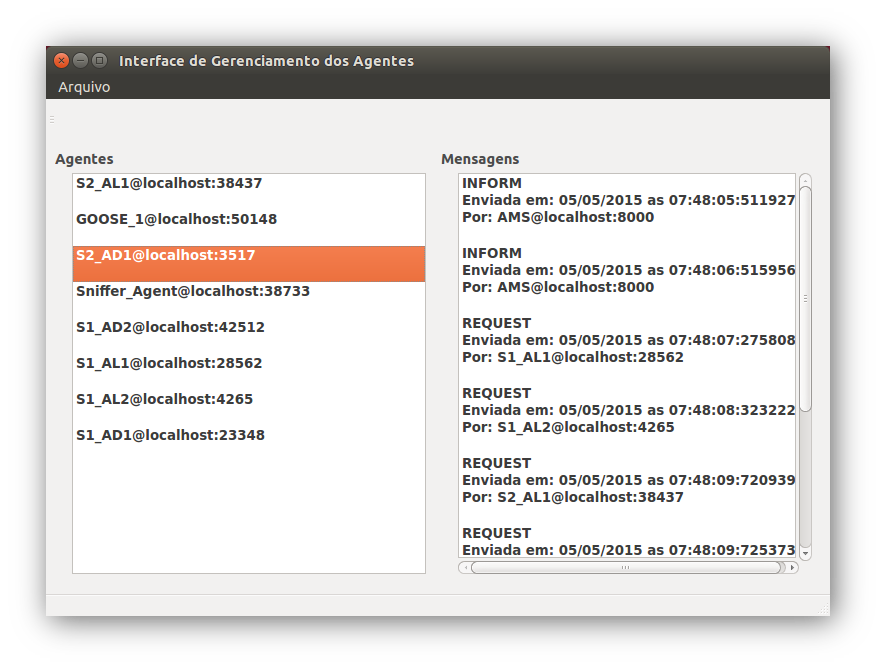
\includegraphics[width=5.0in]{InterfaceSniffer.png}
\end{figure}


\section{Meu Primeiro Agente}
\label{user/meu-primeiro-agente:meu-primeiro-agente}\label{user/meu-primeiro-agente::doc}
Agora já está na hora de construir um agente de verdade!


\subsection{Construindo meu primeiro agente}
\label{user/meu-primeiro-agente:construindo-meu-primeiro-agente}
Para implementar seu primeiro agente abra seu editor de textos preferido e digite o seguinte código:

\begin{Verbatim}[commandchars=\\\{\}]
\PYG{k+kn}{from} \PYG{n+nn}{pade.misc.utility} \PYG{k+kn}{import} \PYG{n}{display\PYGZus{}message}
\PYG{k+kn}{from} \PYG{n+nn}{pade.misc.common} \PYG{k+kn}{import} \PYG{n}{set\PYGZus{}ams}\PYG{p}{,} \PYG{n}{start\PYGZus{}loop}
\PYG{k+kn}{from} \PYG{n+nn}{pade.core.agent} \PYG{k+kn}{import} \PYG{n}{Agent}
\PYG{k+kn}{from} \PYG{n+nn}{pade.acl.aid} \PYG{k+kn}{import} \PYG{n}{AID}


\PYG{k}{class} \PYG{n+nc}{AgenteHelloWorld}\PYG{p}{(}\PYG{n}{Agent}\PYG{p}{)}\PYG{p}{:}
    \PYG{k}{def} \PYG{n+nf}{\PYGZus{}\PYGZus{}init\PYGZus{}\PYGZus{}}\PYG{p}{(}\PYG{n+nb+bp}{self}\PYG{p}{,} \PYG{n}{aid}\PYG{p}{)}\PYG{p}{:}
        \PYG{n+nb}{super}\PYG{p}{(}\PYG{n}{AgenteHelloWorld}\PYG{p}{,} \PYG{n+nb+bp}{self}\PYG{p}{)}\PYG{o}{.}\PYG{n}{\PYGZus{}\PYGZus{}init\PYGZus{}\PYGZus{}}\PYG{p}{(}\PYG{n}{aid}\PYG{o}{=}\PYG{n}{aid}\PYG{p}{,} \PYG{n}{debug}\PYG{o}{=}\PYG{n+nb+bp}{False}\PYG{p}{)}
        \PYG{n}{display\PYGZus{}message}\PYG{p}{(}\PYG{n+nb+bp}{self}\PYG{o}{.}\PYG{n}{aid}\PYG{o}{.}\PYG{n}{localname}\PYG{p}{,} \PYG{l+s}{\PYGZsq{}}\PYG{l+s}{Hello World!}\PYG{l+s}{\PYGZsq{}}\PYG{p}{)}

\PYG{k}{if} \PYG{n}{\PYGZus{}\PYGZus{}name\PYGZus{}\PYGZus{}} \PYG{o}{==} \PYG{l+s}{\PYGZsq{}}\PYG{l+s}{\PYGZus{}\PYGZus{}main\PYGZus{}\PYGZus{}}\PYG{l+s}{\PYGZsq{}}\PYG{p}{:}

    \PYG{n}{set\PYGZus{}ams}\PYG{p}{(}\PYG{l+s}{\PYGZsq{}}\PYG{l+s}{localhost}\PYG{l+s}{\PYGZsq{}}\PYG{p}{,} \PYG{l+m+mi}{8000}\PYG{p}{,} \PYG{n}{debug}\PYG{o}{=}\PYG{n+nb+bp}{False}\PYG{p}{)}

    \PYG{n}{agents} \PYG{o}{=} \PYG{n+nb}{list}\PYG{p}{(}\PYG{p}{)}

    \PYG{n}{agente\PYGZus{}hello} \PYG{o}{=} \PYG{n}{AgenteHelloWorld}\PYG{p}{(}\PYG{n}{AID}\PYG{p}{(}\PYG{n}{name}\PYG{o}{=}\PYG{l+s}{\PYGZsq{}}\PYG{l+s}{agente\PYGZus{}hello}\PYG{l+s}{\PYGZsq{}}\PYG{p}{)}\PYG{p}{)}
    \PYG{n}{agente\PYGZus{}hello}\PYG{o}{.}\PYG{n}{ams} \PYG{o}{=} \PYG{p}{\PYGZob{}}\PYG{l+s}{\PYGZsq{}}\PYG{l+s}{name}\PYG{l+s}{\PYGZsq{}}\PYG{p}{:} \PYG{l+s}{\PYGZsq{}}\PYG{l+s}{localhost}\PYG{l+s}{\PYGZsq{}}\PYG{p}{,} \PYG{l+s}{\PYGZsq{}}\PYG{l+s}{port}\PYG{l+s}{\PYGZsq{}}\PYG{p}{:} \PYG{l+m+mi}{8000}\PYG{p}{\PYGZcb{}}
    \PYG{n}{agents}\PYG{o}{.}\PYG{n}{append}\PYG{p}{(}\PYG{n}{agente\PYGZus{}hello}\PYG{p}{)}

    \PYG{n}{start\PYGZus{}loop}\PYG{p}{(}\PYG{n}{agents}\PYG{p}{,} \PYG{n}{gui}\PYG{o}{=}\PYG{n+nb+bp}{True}\PYG{p}{)}
\end{Verbatim}

Este já é um agente, mas não tem muita utilidade, não é mesmo! Executa apenas uma vez :(

Então como construir um agente que tenha seu comportamento executado de tempos em tempos?


\section{Agentes Temporais}
\label{user/agentes-temporais::doc}\label{user/agentes-temporais:agentes-temporais}
Em aplicações reais é comum que o comportamento do agente seja executado de tempos em tempos e não apenas uma vez, mas como fazer isso no PADE? :(


\subsection{Execução de um agente temporal}
\label{user/agentes-temporais:execucao-de-um-agente-temporal}
Este é um exemplo de um agente que executa indefinidamente um comportamento a cada 1,0 segundos:

\begin{Verbatim}[commandchars=\\\{\}]
\PYG{c}{\PYGZsh{}!coding=utf\PYGZhy{}8}
\PYG{c}{\PYGZsh{} Hello world temporal in PADE!}
\PYG{c}{\PYGZsh{}}
\PYG{c}{\PYGZsh{} Criado por Lucas S Melo em 21 de julho de 2015 \PYGZhy{} Fortaleza, Ceará \PYGZhy{} Brasil}

\PYG{k+kn}{from} \PYG{n+nn}{pade.behaviours.protocols} \PYG{k+kn}{import} \PYG{n}{TimedBehaviour}
\PYG{k+kn}{from} \PYG{n+nn}{pade.misc.utility} \PYG{k+kn}{import} \PYG{n}{display\PYGZus{}message}
\PYG{k+kn}{from} \PYG{n+nn}{pade.misc.common} \PYG{k+kn}{import} \PYG{n}{set\PYGZus{}ams}\PYG{p}{,} \PYG{n}{start\PYGZus{}loop}
\PYG{k+kn}{from} \PYG{n+nn}{pade.core.agent} \PYG{k+kn}{import} \PYG{n}{Agent}
\PYG{k+kn}{from} \PYG{n+nn}{pade.acl.aid} \PYG{k+kn}{import} \PYG{n}{AID}


\PYG{k}{class} \PYG{n+nc}{ComportTemporal}\PYG{p}{(}\PYG{n}{TimedBehaviour}\PYG{p}{)}\PYG{p}{:}
    \PYG{k}{def} \PYG{n+nf}{\PYGZus{}\PYGZus{}init\PYGZus{}\PYGZus{}}\PYG{p}{(}\PYG{n+nb+bp}{self}\PYG{p}{,} \PYG{n}{agent}\PYG{p}{,} \PYG{n}{time}\PYG{p}{)}\PYG{p}{:}
        \PYG{n+nb}{super}\PYG{p}{(}\PYG{n}{ComportTemporal}\PYG{p}{,} \PYG{n+nb+bp}{self}\PYG{p}{)}\PYG{o}{.}\PYG{n}{\PYGZus{}\PYGZus{}init\PYGZus{}\PYGZus{}}\PYG{p}{(}\PYG{n}{agent}\PYG{p}{,} \PYG{n}{time}\PYG{p}{)}

    \PYG{k}{def} \PYG{n+nf}{on\PYGZus{}time}\PYG{p}{(}\PYG{n+nb+bp}{self}\PYG{p}{)}\PYG{p}{:}
        \PYG{n+nb}{super}\PYG{p}{(}\PYG{n}{ComportTemporal}\PYG{p}{,} \PYG{n+nb+bp}{self}\PYG{p}{)}\PYG{o}{.}\PYG{n}{on\PYGZus{}time}\PYG{p}{(}\PYG{p}{)}
        \PYG{n}{display\PYGZus{}message}\PYG{p}{(}\PYG{n+nb+bp}{self}\PYG{o}{.}\PYG{n}{agent}\PYG{o}{.}\PYG{n}{aid}\PYG{o}{.}\PYG{n}{localname}\PYG{p}{,} \PYG{l+s}{\PYGZsq{}}\PYG{l+s}{Hello World!}\PYG{l+s}{\PYGZsq{}}\PYG{p}{)}


\PYG{k}{class} \PYG{n+nc}{AgenteHelloWorld}\PYG{p}{(}\PYG{n}{Agent}\PYG{p}{)}\PYG{p}{:}
    \PYG{k}{def} \PYG{n+nf}{\PYGZus{}\PYGZus{}init\PYGZus{}\PYGZus{}}\PYG{p}{(}\PYG{n+nb+bp}{self}\PYG{p}{,} \PYG{n}{aid}\PYG{p}{)}\PYG{p}{:}
        \PYG{n+nb}{super}\PYG{p}{(}\PYG{n}{AgenteHelloWorld}\PYG{p}{,} \PYG{n+nb+bp}{self}\PYG{p}{)}\PYG{o}{.}\PYG{n}{\PYGZus{}\PYGZus{}init\PYGZus{}\PYGZus{}}\PYG{p}{(}\PYG{n}{aid}\PYG{o}{=}\PYG{n}{aid}\PYG{p}{,} \PYG{n}{debug}\PYG{o}{=}\PYG{n+nb+bp}{False}\PYG{p}{)}

        \PYG{n}{comp\PYGZus{}temp} \PYG{o}{=} \PYG{n}{ComportTemporal}\PYG{p}{(}\PYG{n+nb+bp}{self}\PYG{p}{,} \PYG{l+m+mf}{1.0}\PYG{p}{)}

        \PYG{n+nb+bp}{self}\PYG{o}{.}\PYG{n}{behaviours}\PYG{o}{.}\PYG{n}{append}\PYG{p}{(}\PYG{n}{comp\PYGZus{}temp}\PYG{p}{)}


\PYG{k}{if} \PYG{n}{\PYGZus{}\PYGZus{}name\PYGZus{}\PYGZus{}} \PYG{o}{==} \PYG{l+s}{\PYGZsq{}}\PYG{l+s}{\PYGZus{}\PYGZus{}main\PYGZus{}\PYGZus{}}\PYG{l+s}{\PYGZsq{}}\PYG{p}{:}

    \PYG{n}{set\PYGZus{}ams}\PYG{p}{(}\PYG{l+s}{\PYGZsq{}}\PYG{l+s}{localhost}\PYG{l+s}{\PYGZsq{}}\PYG{p}{,} \PYG{l+m+mi}{8000}\PYG{p}{,} \PYG{n}{debug}\PYG{o}{=}\PYG{n+nb+bp}{False}\PYG{p}{)}

    \PYG{n}{agents} \PYG{o}{=} \PYG{n+nb}{list}\PYG{p}{(}\PYG{p}{)}

    \PYG{n}{agente\PYGZus{}1} \PYG{o}{=} \PYG{n}{AgenteHelloWorld}\PYG{p}{(}\PYG{n}{AID}\PYG{p}{(}\PYG{n}{name}\PYG{o}{=}\PYG{l+s}{\PYGZsq{}}\PYG{l+s}{agente\PYGZus{}1}\PYG{l+s}{\PYGZsq{}}\PYG{p}{)}\PYG{p}{)}
    \PYG{n}{agente\PYGZus{}1}\PYG{o}{.}\PYG{n}{ams} \PYG{o}{=} \PYG{p}{\PYGZob{}}\PYG{l+s}{\PYGZsq{}}\PYG{l+s}{name}\PYG{l+s}{\PYGZsq{}}\PYG{p}{:} \PYG{l+s}{\PYGZsq{}}\PYG{l+s}{localhost}\PYG{l+s}{\PYGZsq{}}\PYG{p}{,} \PYG{l+s}{\PYGZsq{}}\PYG{l+s}{port}\PYG{l+s}{\PYGZsq{}}\PYG{p}{:} \PYG{l+m+mi}{8000}\PYG{p}{\PYGZcb{}}

    \PYG{n}{agents}\PYG{o}{.}\PYG{n}{append}\PYG{p}{(}\PYG{n}{agente\PYGZus{}1}\PYG{p}{)}

    \PYG{n}{start\PYGZus{}loop}\PYG{p}{(}\PYG{n}{agents}\PYG{p}{,} \PYG{n}{gui}\PYG{o}{=}\PYG{n+nb+bp}{True}\PYG{p}{)}
\end{Verbatim}


\subsection{Execução de dois agentes temporais}
\label{user/agentes-temporais:execucao-de-dois-agentes-temporais}
Mas e se eu quiser dois agentes com o mesmo comportamento!? Não tem problema, basta instanciar um outro agente com a mesma classe!

\begin{Verbatim}[commandchars=\\\{\}]
\PYG{k}{if} \PYG{n}{\PYGZus{}\PYGZus{}name\PYGZus{}\PYGZus{}} \PYG{o}{==} \PYG{l+s}{\PYGZsq{}}\PYG{l+s}{\PYGZus{}\PYGZus{}main\PYGZus{}\PYGZus{}}\PYG{l+s}{\PYGZsq{}}\PYG{p}{:}

    \PYG{n}{set\PYGZus{}ams}\PYG{p}{(}\PYG{l+s}{\PYGZsq{}}\PYG{l+s}{localhost}\PYG{l+s}{\PYGZsq{}}\PYG{p}{,} \PYG{l+m+mi}{8000}\PYG{p}{,} \PYG{n}{debug}\PYG{o}{=}\PYG{n+nb+bp}{False}\PYG{p}{)}

    \PYG{n}{agents} \PYG{o}{=} \PYG{n+nb}{list}\PYG{p}{(}\PYG{p}{)}

    \PYG{n}{agente\PYGZus{}1} \PYG{o}{=} \PYG{n}{AgenteHelloWorld}\PYG{p}{(}\PYG{n}{AID}\PYG{p}{(}\PYG{n}{name}\PYG{o}{=}\PYG{l+s}{\PYGZsq{}}\PYG{l+s}{agente\PYGZus{}1}\PYG{l+s}{\PYGZsq{}}\PYG{p}{)}\PYG{p}{)}
    \PYG{n}{agente\PYGZus{}1}\PYG{o}{.}\PYG{n}{ams} \PYG{o}{=} \PYG{p}{\PYGZob{}}\PYG{l+s}{\PYGZsq{}}\PYG{l+s}{name}\PYG{l+s}{\PYGZsq{}}\PYG{p}{:} \PYG{l+s}{\PYGZsq{}}\PYG{l+s}{localhost}\PYG{l+s}{\PYGZsq{}}\PYG{p}{,} \PYG{l+s}{\PYGZsq{}}\PYG{l+s}{port}\PYG{l+s}{\PYGZsq{}}\PYG{p}{:} \PYG{l+m+mi}{8000}\PYG{p}{\PYGZcb{}}

    \PYG{n}{agente\PYGZus{}2} \PYG{o}{=} \PYG{n}{AgenteHelloWorld}\PYG{p}{(}\PYG{n}{AID}\PYG{p}{(}\PYG{n}{name}\PYG{o}{=}\PYG{l+s}{\PYGZsq{}}\PYG{l+s}{agente\PYGZus{}2}\PYG{l+s}{\PYGZsq{}}\PYG{p}{)}\PYG{p}{)}
    \PYG{n}{agente\PYGZus{}2}\PYG{o}{.}\PYG{n}{ams} \PYG{o}{=} \PYG{p}{\PYGZob{}}\PYG{l+s}{\PYGZsq{}}\PYG{l+s}{name}\PYG{l+s}{\PYGZsq{}}\PYG{p}{:} \PYG{l+s}{\PYGZsq{}}\PYG{l+s}{localhost}\PYG{l+s}{\PYGZsq{}}\PYG{p}{,} \PYG{l+s}{\PYGZsq{}}\PYG{l+s}{port}\PYG{l+s}{\PYGZsq{}}\PYG{p}{:} \PYG{l+m+mi}{8000}\PYG{p}{\PYGZcb{}}

    \PYG{n}{agents}\PYG{o}{.}\PYG{n}{append}\PYG{p}{(}\PYG{n}{agente\PYGZus{}1}\PYG{p}{)}
    \PYG{n}{agents}\PYG{o}{.}\PYG{n}{append}\PYG{p}{(}\PYG{n}{agente\PYGZus{}2}\PYG{p}{)}

    \PYG{n}{start\PYGZus{}loop}\PYG{p}{(}\PYG{n}{agents}\PYG{p}{,} \PYG{n}{gui}\PYG{o}{=}\PYG{n+nb+bp}{True}\PYG{p}{)}
\end{Verbatim}


\section{Enviando Mensagens}
\label{user/enviando-mensagens:enviando-mensagens}\label{user/enviando-mensagens::doc}
Para enviar uma mensagem com o PADE é muito simples! As mensagens enviadas pelos agentes desenvolvidos com PADE seguem o padrão FIPA-ACL e têm os seguintes campos:
\begin{itemize}
\item {} 
\emph{conversation-id:} identidade única de uma conversa;

\item {} 
\emph{performative:} rótulo da mensagem;

\item {} 
\emph{sender:} remetente da mensagem;

\item {} 
\emph{receivers:} destinatários da mensagem;

\item {} 
\emph{content:} conteúdo da mensagem;

\item {} 
\emph{protocol:} protocolo da mensagem;

\item {} 
\emph{language:} linguagem utilizada;

\item {} 
\emph{encoding:} codificação da mensagem;

\item {} 
\emph{ontology:} ontologia utilizada;

\item {} 
\emph{reply-with:} Expressão utilizada pelo agente de resposta a identificar a mensagem;

\item {} 
\emph{reply-by:} A referência a uma ação anterior em que a mensagem é uma resposta;

\item {} 
\emph{in-reply-to:} Data/hora indicando quando uma resposta deve ser recebida..

\end{itemize}


\subsection{Mensagens FIPA-ACL no PADE}
\label{user/enviando-mensagens:mensagens-fipa-acl-no-pade}
Uma mensagem FIPA-ACL pode ser montada no pade da seguinte forma:

\begin{Verbatim}[commandchars=\\\{\}]
\PYG{k+kn}{from} \PYG{n+nn}{pade.acl.messages} \PYG{k+kn}{import} \PYG{n}{ACLMessage}\PYG{p}{,} \PYG{n}{AID}
\PYG{n}{message} \PYG{o}{=} \PYG{n}{ACLMessage}\PYG{p}{(}\PYG{n}{ACLMessage}\PYG{o}{.}\PYG{n}{INFORM}\PYG{p}{)}
\PYG{n}{message}\PYG{o}{.}\PYG{n}{set\PYGZus{}protocol}\PYG{p}{(}\PYG{n}{ACLMessage}\PYG{o}{.}\PYG{n}{FIPA\PYGZus{}REQUEST\PYGZus{}PROTOCOL}\PYG{p}{)}
\PYG{n}{message}\PYG{o}{.}\PYG{n}{add\PYGZus{}receiver}\PYG{p}{(}\PYG{n}{AID}\PYG{p}{(}\PYG{l+s}{\PYGZsq{}}\PYG{l+s}{agente\PYGZus{}destino}\PYG{l+s}{\PYGZsq{}}\PYG{p}{)}\PYG{p}{)}
\PYG{n}{message}\PYG{o}{.}\PYG{n}{set\PYGZus{}content}\PYG{p}{(}\PYG{l+s}{\PYGZsq{}}\PYG{l+s}{Ola Agente}\PYG{l+s}{\PYGZsq{}}\PYG{p}{)}
\end{Verbatim}


\subsection{Enviando uma mensagem com PADE}
\label{user/enviando-mensagens:enviando-uma-mensagem-com-pade}
Uma vez que se está dentro de uma instância da classe \emph{Agent()} a mensagem pode ser enviada, simplesmente utilizando o comando:

\begin{Verbatim}[commandchars=\\\{\}]
\PYG{n+nb+bp}{self}\PYG{o}{.}\PYG{n}{send}\PYG{p}{(}\PYG{n}{message}\PYG{p}{)}
\end{Verbatim}


\subsection{Mensagem no padrão FIPA-ACL}
\label{user/enviando-mensagens:mensagem-no-padrao-fipa-acl}
Realizando o comando \emph{print message} a mensagem no padão FIPA ACL será impressa na tela:

\begin{Verbatim}[commandchars=\\\{\}]
(inform
    :conversationID b2e806b8\PYGZhy{}50a0\PYGZhy{}11e5\PYGZhy{}b3b6\PYGZhy{}e8b1fc5c3cdf
    :receiver
        (set
            (agent\PYGZhy{}identifier
                :name agente\PYGZus{}destino@localhost:51645
                :addresses
                    (sequence
                    localhost:51645
                    )
            )

        )
    :content \PYGZdq{}Ola Agente\PYGZdq{}
    :protocol fipa\PYGZhy{}request protocol
)
\end{Verbatim}


\subsection{Mensagem no padrão XML}
\label{user/enviando-mensagens:mensagem-no-padrao-xml}
Mas também é possível obter a mensagem no formato XML por meio do comando \emph{print message.as\_xml()}

\begin{Verbatim}[commandchars=\\\{\}]
\PYG{c+cp}{\PYGZlt{}?xml version=\PYGZdq{}1.0\PYGZdq{} ?\PYGZgt{}}
\PYG{n+nt}{\PYGZlt{}ACLMessage} \PYG{n+na}{date=}\PYG{l+s}{\PYGZdq{}01/09/2015 as 08:58:03:113891\PYGZdq{}}\PYG{n+nt}{\PYGZgt{}}
        \PYG{n+nt}{\PYGZlt{}performative}\PYG{n+nt}{\PYGZgt{}}inform\PYG{n+nt}{\PYGZlt{}/performative\PYGZgt{}}
        \PYG{n+nt}{\PYGZlt{}sender}\PYG{n+nt}{/\PYGZgt{}}
        \PYG{n+nt}{\PYGZlt{}receivers}\PYG{n+nt}{\PYGZgt{}}
                \PYG{n+nt}{\PYGZlt{}receiver}\PYG{n+nt}{\PYGZgt{}}agente\PYGZus{}destino@localhost:51645\PYG{n+nt}{\PYGZlt{}/receiver\PYGZgt{}}
        \PYG{n+nt}{\PYGZlt{}/receivers\PYGZgt{}}
        \PYG{n+nt}{\PYGZlt{}reply\PYGZhy{}to}\PYG{n+nt}{/\PYGZgt{}}
        \PYG{n+nt}{\PYGZlt{}content}\PYG{n+nt}{\PYGZgt{}}Ola Agente\PYG{n+nt}{\PYGZlt{}/content\PYGZgt{}}
        \PYG{n+nt}{\PYGZlt{}language}\PYG{n+nt}{/\PYGZgt{}}
        \PYG{n+nt}{\PYGZlt{}enconding}\PYG{n+nt}{/\PYGZgt{}}
        \PYG{n+nt}{\PYGZlt{}ontology}\PYG{n+nt}{/\PYGZgt{}}
        \PYG{n+nt}{\PYGZlt{}protocol}\PYG{n+nt}{\PYGZgt{}}fipa\PYGZhy{}request protocol\PYG{n+nt}{\PYGZlt{}/protocol\PYGZgt{}}
        \PYG{n+nt}{\PYGZlt{}conversationID}\PYG{n+nt}{\PYGZgt{}}b2e806b8\PYGZhy{}50a0\PYGZhy{}11e5\PYGZhy{}b3b6\PYGZhy{}e8b1fc5c3cdf\PYG{n+nt}{\PYGZlt{}/conversationID\PYGZgt{}}
        \PYG{n+nt}{\PYGZlt{}reply\PYGZhy{}with}\PYG{n+nt}{/\PYGZgt{}}
        \PYG{n+nt}{\PYGZlt{}in\PYGZhy{}reply\PYGZhy{}to}\PYG{n+nt}{/\PYGZgt{}}
        \PYG{n+nt}{\PYGZlt{}reply\PYGZhy{}by}\PYG{n+nt}{/\PYGZgt{}}
\PYG{n+nt}{\PYGZlt{}/ACLMessage\PYGZgt{}}
\end{Verbatim}


\section{Recebendo Mensagens}
\label{user/recebendo-mensagens:recebendo-mensagens}\label{user/recebendo-mensagens::doc}
No PADE para que um agente possa receber mensagens, basta que o método react() seja implementado, dentro da classe que herda da classe \emph{Agent()}.


\subsection{Recebendo mensagens FIPA-ACL com PADE}
\label{user/recebendo-mensagens:recebendo-mensagens-fipa-acl-com-pade}
No exemplo a seguir são implementados dois agentes distintos, o primeiro é o agente \code{{}`remetente{}`} modelado pela classe \emph{Remetente()}, que tem o papel de enviar uma mensagem ao agente \emph{destinatario} modelado pela classe \emph{Destinatario}, que irá receber a mensagem enviada pelo agente \emph{remetente} e por isso tem o método \emph{react()} implementado.

\begin{Verbatim}[commandchars=\\\{\}]
\PYG{k+kn}{from} \PYG{n+nn}{pade.misc.utility} \PYG{k+kn}{import} \PYG{n}{display\PYGZus{}message}
\PYG{k+kn}{from} \PYG{n+nn}{pade.misc.common} \PYG{k+kn}{import} \PYG{n}{set\PYGZus{}ams}\PYG{p}{,} \PYG{n}{start\PYGZus{}loop}
\PYG{k+kn}{from} \PYG{n+nn}{pade.core.agent} \PYG{k+kn}{import} \PYG{n}{Agent}
\PYG{k+kn}{from} \PYG{n+nn}{pade.acl.aid} \PYG{k+kn}{import} \PYG{n}{AID}
\PYG{k+kn}{from} \PYG{n+nn}{pade.acl.messages} \PYG{k+kn}{import} \PYG{n}{ACLMessage}


\PYG{k}{class} \PYG{n+nc}{Remetente}\PYG{p}{(}\PYG{n}{Agent}\PYG{p}{)}\PYG{p}{:}
    \PYG{k}{def} \PYG{n+nf}{\PYGZus{}\PYGZus{}init\PYGZus{}\PYGZus{}}\PYG{p}{(}\PYG{n+nb+bp}{self}\PYG{p}{,} \PYG{n}{aid}\PYG{p}{)}\PYG{p}{:}
        \PYG{n+nb}{super}\PYG{p}{(}\PYG{n}{Remetente}\PYG{p}{,} \PYG{n+nb+bp}{self}\PYG{p}{)}\PYG{o}{.}\PYG{n}{\PYGZus{}\PYGZus{}init\PYGZus{}\PYGZus{}}\PYG{p}{(}\PYG{n}{aid}\PYG{o}{=}\PYG{n}{aid}\PYG{p}{,} \PYG{n}{debug}\PYG{o}{=}\PYG{n+nb+bp}{False}\PYG{p}{)}

    \PYG{k}{def} \PYG{n+nf}{on\PYGZus{}start}\PYG{p}{(}\PYG{n+nb+bp}{self}\PYG{p}{)}\PYG{p}{:}
        \PYG{n}{display\PYGZus{}message}\PYG{p}{(}\PYG{n+nb+bp}{self}\PYG{o}{.}\PYG{n}{aid}\PYG{o}{.}\PYG{n}{localname}\PYG{p}{,} \PYG{l+s}{\PYGZsq{}}\PYG{l+s}{Enviando Mensagem}\PYG{l+s}{\PYGZsq{}}\PYG{p}{)}
        \PYG{n}{message} \PYG{o}{=} \PYG{n}{ACLMessage}\PYG{p}{(}\PYG{n}{ACLMessage}\PYG{o}{.}\PYG{n}{INFORM}\PYG{p}{)}
        \PYG{n}{message}\PYG{o}{.}\PYG{n}{add\PYGZus{}receiver}\PYG{p}{(}\PYG{n}{AID}\PYG{p}{(}\PYG{l+s}{\PYGZsq{}}\PYG{l+s}{destinatario}\PYG{l+s}{\PYGZsq{}}\PYG{p}{)}\PYG{p}{)}
        \PYG{n}{message}\PYG{o}{.}\PYG{n}{set\PYGZus{}content}\PYG{p}{(}\PYG{l+s}{\PYGZsq{}}\PYG{l+s}{Ola}\PYG{l+s}{\PYGZsq{}}\PYG{p}{)}
        \PYG{n+nb+bp}{self}\PYG{o}{.}\PYG{n}{send}\PYG{p}{(}\PYG{n}{message}\PYG{p}{)}

    \PYG{k}{def} \PYG{n+nf}{react}\PYG{p}{(}\PYG{n+nb+bp}{self}\PYG{p}{,} \PYG{n}{message}\PYG{p}{)}\PYG{p}{:}
        \PYG{k}{pass}


\PYG{k}{class} \PYG{n+nc}{Destinatario}\PYG{p}{(}\PYG{n}{Agent}\PYG{p}{)}\PYG{p}{:}
    \PYG{k}{def} \PYG{n+nf}{\PYGZus{}\PYGZus{}init\PYGZus{}\PYGZus{}}\PYG{p}{(}\PYG{n+nb+bp}{self}\PYG{p}{,} \PYG{n}{aid}\PYG{p}{)}\PYG{p}{:}
        \PYG{n+nb}{super}\PYG{p}{(}\PYG{n}{Destinatario}\PYG{p}{,} \PYG{n+nb+bp}{self}\PYG{p}{)}\PYG{o}{.}\PYG{n}{\PYGZus{}\PYGZus{}init\PYGZus{}\PYGZus{}}\PYG{p}{(}\PYG{n}{aid}\PYG{o}{=}\PYG{n}{aid}\PYG{p}{,} \PYG{n}{debug}\PYG{o}{=}\PYG{n+nb+bp}{False}\PYG{p}{)}

    \PYG{k}{def} \PYG{n+nf}{react}\PYG{p}{(}\PYG{n+nb+bp}{self}\PYG{p}{,} \PYG{n}{message}\PYG{p}{)}\PYG{p}{:}
        \PYG{n}{display\PYGZus{}message}\PYG{p}{(}\PYG{n+nb+bp}{self}\PYG{o}{.}\PYG{n}{aid}\PYG{o}{.}\PYG{n}{localname}\PYG{p}{,} \PYG{l+s}{\PYGZsq{}}\PYG{l+s}{Mensagem recebida}\PYG{l+s}{\PYGZsq{}}\PYG{p}{)}


\PYG{k}{if} \PYG{n}{\PYGZus{}\PYGZus{}name\PYGZus{}\PYGZus{}} \PYG{o}{==} \PYG{l+s}{\PYGZsq{}}\PYG{l+s}{\PYGZus{}\PYGZus{}main\PYGZus{}\PYGZus{}}\PYG{l+s}{\PYGZsq{}}\PYG{p}{:}

    \PYG{n}{set\PYGZus{}ams}\PYG{p}{(}\PYG{l+s}{\PYGZsq{}}\PYG{l+s}{localhost}\PYG{l+s}{\PYGZsq{}}\PYG{p}{,} \PYG{l+m+mi}{8000}\PYG{p}{,} \PYG{n}{debug}\PYG{o}{=}\PYG{n+nb+bp}{False}\PYG{p}{)}

    \PYG{n}{agentes} \PYG{o}{=} \PYG{n+nb}{list}\PYG{p}{(}\PYG{p}{)}

    \PYG{n}{destinatario} \PYG{o}{=} \PYG{n}{Destinatario}\PYG{p}{(}\PYG{n}{AID}\PYG{p}{(}\PYG{n}{name}\PYG{o}{=}\PYG{l+s}{\PYGZsq{}}\PYG{l+s}{destinatario}\PYG{l+s}{\PYGZsq{}}\PYG{p}{)}\PYG{p}{)}
    \PYG{n}{destinatario}\PYG{o}{.}\PYG{n}{ams} \PYG{o}{=} \PYG{p}{\PYGZob{}}\PYG{l+s}{\PYGZsq{}}\PYG{l+s}{name}\PYG{l+s}{\PYGZsq{}}\PYG{p}{:} \PYG{l+s}{\PYGZsq{}}\PYG{l+s}{localhost}\PYG{l+s}{\PYGZsq{}}\PYG{p}{,} \PYG{l+s}{\PYGZsq{}}\PYG{l+s}{port}\PYG{l+s}{\PYGZsq{}}\PYG{p}{:} \PYG{l+m+mi}{8000}\PYG{p}{\PYGZcb{}}
    \PYG{n}{agentes}\PYG{o}{.}\PYG{n}{append}\PYG{p}{(}\PYG{n}{destinatario}\PYG{p}{)}

    \PYG{n}{remetente} \PYG{o}{=} \PYG{n}{Remetente}\PYG{p}{(}\PYG{n}{AID}\PYG{p}{(}\PYG{n}{name}\PYG{o}{=}\PYG{l+s}{\PYGZsq{}}\PYG{l+s}{remetente}\PYG{l+s}{\PYGZsq{}}\PYG{p}{)}\PYG{p}{)}
    \PYG{n}{remetente}\PYG{o}{.}\PYG{n}{ams} \PYG{o}{=} \PYG{p}{\PYGZob{}}\PYG{l+s}{\PYGZsq{}}\PYG{l+s}{name}\PYG{l+s}{\PYGZsq{}}\PYG{p}{:} \PYG{l+s}{\PYGZsq{}}\PYG{l+s}{localhost}\PYG{l+s}{\PYGZsq{}}\PYG{p}{,} \PYG{l+s}{\PYGZsq{}}\PYG{l+s}{port}\PYG{l+s}{\PYGZsq{}}\PYG{p}{:} \PYG{l+m+mi}{8000}\PYG{p}{\PYGZcb{}}
    \PYG{n}{agentes}\PYG{o}{.}\PYG{n}{append}\PYG{p}{(}\PYG{n}{remetente}\PYG{p}{)}

    \PYG{n}{start\PYGZus{}loop}\PYG{p}{(}\PYG{n}{agentes}\PYG{p}{,} \PYG{n}{gui}\PYG{o}{=}\PYG{n+nb+bp}{True}\PYG{p}{)}
\end{Verbatim}


\subsection{Visualização via Interface Gráfica}
\label{user/recebendo-mensagens:visualizacao-via-interface-grafica}
A seguir é possível observar a interface gráfica do PADE que mostra os agentes cadastrados no AMS.
\begin{figure}[htbp]
\centering

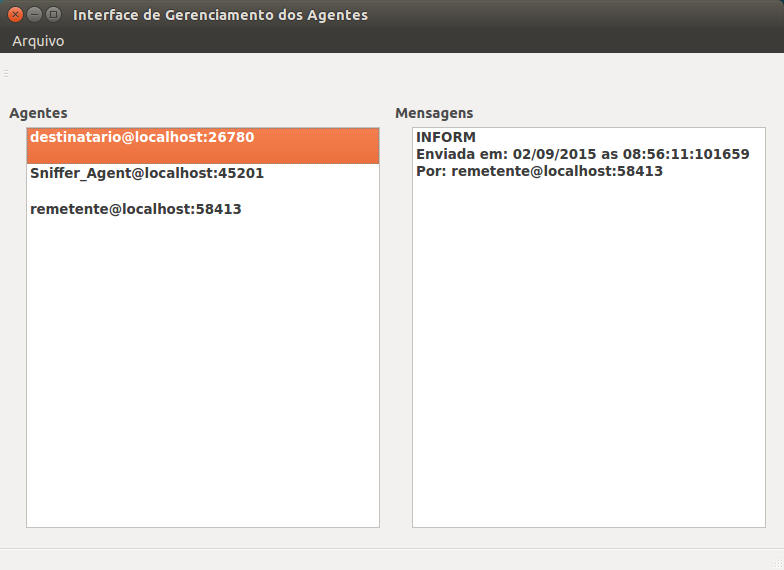
\includegraphics[width=4.5in]{janela_agentes.png}
\end{figure}

Ao clicar na mensagem recebida pelo agente \emph{destinatario} é possível observar todos os dados contidos na mensagem:
\begin{figure}[htbp]
\centering

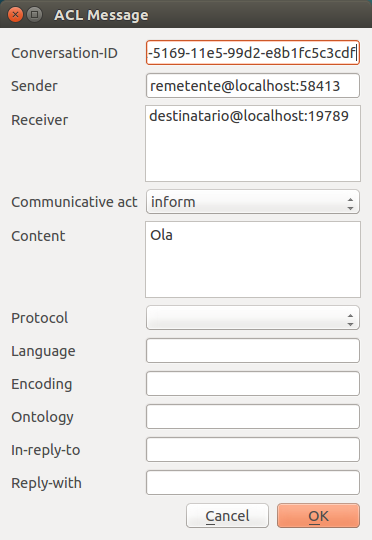
\includegraphics[width=3.0in]{janela_mensagem.png}
\end{figure}


\section{Um momento Por Favor!}
\label{user/um-momento::doc}\label{user/um-momento:um-momento-por-favor}
Com PADE é possível adiar a execução de um determinado trecho de código de forma bem simples! É só utilizar o método \emph{call\_later()} disponível na classe \emph{Agent()}.


\subsection{Como utilizar o método call\_later()}
\label{user/um-momento:como-utilizar-o-metodo-call-later}
Para utilizar \emph{call\_later()}, os seguintes parâmetros devem ser especificados: tempo de atraso, metodo que deve ser chamado após este tempo e argumento do metodo utilizado, \emph{call\_later(tempo, metodo, *args)}.

No código a seguir utiliza \emph{call\_later()} é utilizado na classe \emph{Remetente()} no método \emph{on\_start()} para assegurar que todos os agentes já foram lançados na plataforma, chamando o método \emph{send\_message()} 4,0 segundos após a inicialização dos agentes:

\begin{Verbatim}[commandchars=\\\{\}]
\PYG{k+kn}{from} \PYG{n+nn}{pade.misc.utility} \PYG{k+kn}{import} \PYG{n}{display\PYGZus{}message}
\PYG{k+kn}{from} \PYG{n+nn}{pade.misc.common} \PYG{k+kn}{import} \PYG{n}{set\PYGZus{}ams}\PYG{p}{,} \PYG{n}{start\PYGZus{}loop}
\PYG{k+kn}{from} \PYG{n+nn}{pade.core.agent} \PYG{k+kn}{import} \PYG{n}{Agent}
\PYG{k+kn}{from} \PYG{n+nn}{pade.acl.aid} \PYG{k+kn}{import} \PYG{n}{AID}
\PYG{k+kn}{from} \PYG{n+nn}{pade.acl.messages} \PYG{k+kn}{import} \PYG{n}{ACLMessage}


\PYG{k}{class} \PYG{n+nc}{Remetente}\PYG{p}{(}\PYG{n}{Agent}\PYG{p}{)}\PYG{p}{:}
    \PYG{k}{def} \PYG{n+nf}{\PYGZus{}\PYGZus{}init\PYGZus{}\PYGZus{}}\PYG{p}{(}\PYG{n+nb+bp}{self}\PYG{p}{,} \PYG{n}{aid}\PYG{p}{)}\PYG{p}{:}
        \PYG{n+nb}{super}\PYG{p}{(}\PYG{n}{Remetente}\PYG{p}{,} \PYG{n+nb+bp}{self}\PYG{p}{)}\PYG{o}{.}\PYG{n}{\PYGZus{}\PYGZus{}init\PYGZus{}\PYGZus{}}\PYG{p}{(}\PYG{n}{aid}\PYG{o}{=}\PYG{n}{aid}\PYG{p}{,} \PYG{n}{debug}\PYG{o}{=}\PYG{n+nb+bp}{False}\PYG{p}{)}

    \PYG{k}{def} \PYG{n+nf}{on\PYGZus{}start}\PYG{p}{(}\PYG{n+nb+bp}{self}\PYG{p}{)}\PYG{p}{:}
        \PYG{n+nb+bp}{self}\PYG{o}{.}\PYG{n}{call\PYGZus{}later}\PYG{p}{(}\PYG{l+m+mf}{4.0}\PYG{p}{,} \PYG{n+nb+bp}{self}\PYG{o}{.}\PYG{n}{send\PYGZus{}message}\PYG{p}{)}

    \PYG{k}{def} \PYG{n+nf}{send\PYGZus{}message}\PYG{p}{(}\PYG{n+nb+bp}{self}\PYG{p}{)}\PYG{p}{:}
        \PYG{n}{display\PYGZus{}message}\PYG{p}{(}\PYG{n+nb+bp}{self}\PYG{o}{.}\PYG{n}{aid}\PYG{o}{.}\PYG{n}{localname}\PYG{p}{,} \PYG{l+s}{\PYGZsq{}}\PYG{l+s}{Enviando Mensagem}\PYG{l+s}{\PYGZsq{}}\PYG{p}{)}
        \PYG{n}{message} \PYG{o}{=} \PYG{n}{ACLMessage}\PYG{p}{(}\PYG{n}{ACLMessage}\PYG{o}{.}\PYG{n}{INFORM}\PYG{p}{)}
        \PYG{n}{message}\PYG{o}{.}\PYG{n}{add\PYGZus{}receiver}\PYG{p}{(}\PYG{n}{AID}\PYG{p}{(}\PYG{l+s}{\PYGZsq{}}\PYG{l+s}{destinatario}\PYG{l+s}{\PYGZsq{}}\PYG{p}{)}\PYG{p}{)}
        \PYG{n}{message}\PYG{o}{.}\PYG{n}{set\PYGZus{}content}\PYG{p}{(}\PYG{l+s}{\PYGZsq{}}\PYG{l+s}{Ola}\PYG{l+s}{\PYGZsq{}}\PYG{p}{)}
        \PYG{n+nb+bp}{self}\PYG{o}{.}\PYG{n}{send}\PYG{p}{(}\PYG{n}{message}\PYG{p}{)}

    \PYG{k}{def} \PYG{n+nf}{react}\PYG{p}{(}\PYG{n+nb+bp}{self}\PYG{p}{,} \PYG{n}{message}\PYG{p}{)}\PYG{p}{:}
        \PYG{k}{pass}


\PYG{k}{class} \PYG{n+nc}{Destinatario}\PYG{p}{(}\PYG{n}{Agent}\PYG{p}{)}\PYG{p}{:}
    \PYG{k}{def} \PYG{n+nf}{\PYGZus{}\PYGZus{}init\PYGZus{}\PYGZus{}}\PYG{p}{(}\PYG{n+nb+bp}{self}\PYG{p}{,} \PYG{n}{aid}\PYG{p}{)}\PYG{p}{:}
        \PYG{n+nb}{super}\PYG{p}{(}\PYG{n}{Destinatario}\PYG{p}{,} \PYG{n+nb+bp}{self}\PYG{p}{)}\PYG{o}{.}\PYG{n}{\PYGZus{}\PYGZus{}init\PYGZus{}\PYGZus{}}\PYG{p}{(}\PYG{n}{aid}\PYG{o}{=}\PYG{n}{aid}\PYG{p}{,} \PYG{n}{debug}\PYG{o}{=}\PYG{n+nb+bp}{False}\PYG{p}{)}

    \PYG{k}{def} \PYG{n+nf}{react}\PYG{p}{(}\PYG{n+nb+bp}{self}\PYG{p}{,} \PYG{n}{message}\PYG{p}{)}\PYG{p}{:}
        \PYG{n}{display\PYGZus{}message}\PYG{p}{(}\PYG{n+nb+bp}{self}\PYG{o}{.}\PYG{n}{aid}\PYG{o}{.}\PYG{n}{localname}\PYG{p}{,} \PYG{l+s}{\PYGZsq{}}\PYG{l+s}{Mensagem recebida}\PYG{l+s}{\PYGZsq{}}\PYG{p}{)}


\PYG{k}{if} \PYG{n}{\PYGZus{}\PYGZus{}name\PYGZus{}\PYGZus{}} \PYG{o}{==} \PYG{l+s}{\PYGZsq{}}\PYG{l+s}{\PYGZus{}\PYGZus{}main\PYGZus{}\PYGZus{}}\PYG{l+s}{\PYGZsq{}}\PYG{p}{:}

    \PYG{n}{set\PYGZus{}ams}\PYG{p}{(}\PYG{l+s}{\PYGZsq{}}\PYG{l+s}{localhost}\PYG{l+s}{\PYGZsq{}}\PYG{p}{,} \PYG{l+m+mi}{8000}\PYG{p}{,} \PYG{n}{debug}\PYG{o}{=}\PYG{n+nb+bp}{False}\PYG{p}{)}

    \PYG{n}{agentes} \PYG{o}{=} \PYG{n+nb}{list}\PYG{p}{(}\PYG{p}{)}

    \PYG{n}{destinatario} \PYG{o}{=} \PYG{n}{Destinatario}\PYG{p}{(}\PYG{n}{AID}\PYG{p}{(}\PYG{n}{name}\PYG{o}{=}\PYG{l+s}{\PYGZsq{}}\PYG{l+s}{destinatario}\PYG{l+s}{\PYGZsq{}}\PYG{p}{)}\PYG{p}{)}
    \PYG{n}{destinatario}\PYG{o}{.}\PYG{n}{ams} \PYG{o}{=} \PYG{p}{\PYGZob{}}\PYG{l+s}{\PYGZsq{}}\PYG{l+s}{name}\PYG{l+s}{\PYGZsq{}}\PYG{p}{:} \PYG{l+s}{\PYGZsq{}}\PYG{l+s}{localhost}\PYG{l+s}{\PYGZsq{}}\PYG{p}{,} \PYG{l+s}{\PYGZsq{}}\PYG{l+s}{port}\PYG{l+s}{\PYGZsq{}}\PYG{p}{:} \PYG{l+m+mi}{8000}\PYG{p}{\PYGZcb{}}
    \PYG{n}{agentes}\PYG{o}{.}\PYG{n}{append}\PYG{p}{(}\PYG{n}{destinatario}\PYG{p}{)}

    \PYG{n}{remetente} \PYG{o}{=} \PYG{n}{Remetente}\PYG{p}{(}\PYG{n}{AID}\PYG{p}{(}\PYG{n}{name}\PYG{o}{=}\PYG{l+s}{\PYGZsq{}}\PYG{l+s}{remetente}\PYG{l+s}{\PYGZsq{}}\PYG{p}{)}\PYG{p}{)}
    \PYG{n}{remetente}\PYG{o}{.}\PYG{n}{ams} \PYG{o}{=} \PYG{p}{\PYGZob{}}\PYG{l+s}{\PYGZsq{}}\PYG{l+s}{name}\PYG{l+s}{\PYGZsq{}}\PYG{p}{:} \PYG{l+s}{\PYGZsq{}}\PYG{l+s}{localhost}\PYG{l+s}{\PYGZsq{}}\PYG{p}{,} \PYG{l+s}{\PYGZsq{}}\PYG{l+s}{port}\PYG{l+s}{\PYGZsq{}}\PYG{p}{:} \PYG{l+m+mi}{8000}\PYG{p}{\PYGZcb{}}
    \PYG{n}{agentes}\PYG{o}{.}\PYG{n}{append}\PYG{p}{(}\PYG{n}{remetente}\PYG{p}{)}

    \PYG{n}{start\PYGZus{}loop}\PYG{p}{(}\PYG{n}{agentes}\PYG{p}{,} \PYG{n}{gui}\PYG{o}{=}\PYG{n+nb+bp}{True}\PYG{p}{)}
\end{Verbatim}


\section{Enviando Objetos}
\label{user/enviando-objetos:enviando-objetos}\label{user/enviando-objetos::doc}
Nem sempre o que é preciso enviar para outros agentes pode ser representado por texto simpes não é mesmo!

Para enviar objetos encapsulados no content de mensagens FIPA-ACL com PADE basta utilizar o módulo nativo do Python \emph{pickle}.


\subsection{Enviando objetos serializados com pickle}
\label{user/enviando-objetos:enviando-objetos-serializados-com-pickle}
Para enviar um objeto serializado com piclke basta seguir os passos:

\begin{Verbatim}[commandchars=\\\{\}]
\PYG{k+kn}{import} \PYG{n+nn}{pickle}
\end{Verbatim}

\emph{pickle} é uma biblioteca para serialização de objetos, assim, para serializar um objeto qualquer, utilize \emph{pickle.dumps()}, veja:

\begin{Verbatim}[commandchars=\\\{\}]
\PYG{n}{dados} \PYG{o}{=} \PYG{p}{\PYGZob{}}\PYG{l+s}{\PYGZsq{}}\PYG{l+s}{nome}\PYG{l+s}{\PYGZsq{}} \PYG{p}{:} \PYG{l+s}{\PYGZsq{}}\PYG{l+s}{agente\PYGZus{}consumidor}\PYG{l+s}{\PYGZsq{}}\PYG{p}{,} \PYG{l+s}{\PYGZsq{}}\PYG{l+s}{porta}\PYG{l+s}{\PYGZsq{}} \PYG{p}{:} \PYG{l+m+mi}{2004}\PYG{p}{\PYGZcb{}}
\PYG{n}{dados\PYGZus{}serial} \PYG{o}{=} \PYG{n}{pickle}\PYG{o}{.}\PYG{n}{dumps}\PYG{p}{(}\PYG{n}{dados}\PYG{p}{)}
\PYG{n}{message}\PYG{o}{.}\PYG{n}{set\PYGZus{}content}\PYG{p}{(}\PYG{n}{dados\PYGZus{}serial}\PYG{p}{)}
\end{Verbatim}

Pronto! O objeto já pode ser enviado no conteúdo da mensagem.


\subsection{Recebendo objetos serializados com pickle}
\label{user/enviando-objetos:recebendo-objetos-serializados-com-pickle}
Agora para receber o objeto, basta carregá-lo utilizando o comando:

\begin{Verbatim}[commandchars=\\\{\}]
\PYG{n}{dados\PYGZus{}serial} \PYG{o}{=} \PYG{n}{message}\PYG{o}{.}\PYG{n}{content}
\PYG{n}{dados} \PYG{o}{=} \PYG{n}{pickle}\PYG{o}{.}\PYG{n}{loads}\PYG{p}{(}\PYG{n}{dados\PYGZus{}serial}\PYG{p}{)}
\end{Verbatim}

Simples assim ;)


\section{Seleção de Mensagens}
\label{user/selecao-de-mensagens:selecao-de-mensagens}\label{user/selecao-de-mensagens::doc}
Com PADE é possível implementar filtros de mensagens de maneira simples e direta, por meio da classe Filtro:

\begin{Verbatim}[commandchars=\\\{\}]
\PYG{k+kn}{from} \PYG{n+nn}{pade.acl.filters} \PYG{k+kn}{import} \PYG{n}{Filter}
\end{Verbatim}


\subsection{Filtrando mensagens com o módulo filters}
\label{user/selecao-de-mensagens:filtrando-mensagens-com-o-modulo-filters}
Por exemplo para a seguinte mensagem:

\begin{Verbatim}[commandchars=\\\{\}]
\PYG{k+kn}{from} \PYG{n+nn}{pade.acl.messages} \PYG{k+kn}{import} \PYG{n}{ACLMessage}
\PYG{k+kn}{from} \PYG{n+nn}{pade.acl.aid} \PYG{k+kn}{import} \PYG{n}{AID}

\PYG{n}{message} \PYG{o}{=} \PYG{n}{ACLMessage}\PYG{p}{(}\PYG{n}{ACLMessage}\PYG{o}{.}\PYG{n}{INFORM}\PYG{p}{)}
\PYG{n}{message}\PYG{o}{.}\PYG{n}{set\PYGZus{}protocol}\PYG{p}{(}\PYG{n}{ACLMessage}\PYG{o}{.}\PYG{n}{FIPA\PYGZus{}REQUEST\PYGZus{}PROTOCOL}\PYG{p}{)}
\PYG{n}{message}\PYG{o}{.}\PYG{n}{set\PYGZus{}sender}\PYG{p}{(}\PYG{n}{AID}\PYG{p}{(}\PYG{l+s}{\PYGZsq{}}\PYG{l+s}{remetente}\PYG{l+s}{\PYGZsq{}}\PYG{p}{)}\PYG{p}{)}
\PYG{n}{message}\PYG{o}{.}\PYG{n}{add\PYGZus{}receiver}\PYG{p}{(}\PYG{n}{AID}\PYG{p}{(}\PYG{l+s}{\PYGZsq{}}\PYG{l+s}{destinatario}\PYG{l+s}{\PYGZsq{}}\PYG{p}{)}\PYG{p}{)}
\end{Verbatim}

Podemos criar o seguinte filtro:

\begin{Verbatim}[commandchars=\\\{\}]
\PYG{k+kn}{from} \PYG{n+nn}{pade.acl.filters} \PYG{k+kn}{import} \PYG{n}{Filter}

\PYG{n}{f}\PYG{o}{.}\PYG{n}{performative} \PYG{o}{=} \PYG{n}{ACLMessage}\PYG{o}{.}\PYG{n}{REQUEST}
\end{Verbatim}

Em uma sessão IPython é possível observar o efeito da aplicação do filtro sobre a mensagem:

\begin{Verbatim}[commandchars=\\\{\}]
\PYG{g+gp}{In [12]: }\PYG{n}{f}\PYG{o}{.}\PYG{n}{filter}\PYG{p}{(}\PYG{n}{message}\PYG{p}{)}
\PYG{g+gr}{Out[12]: }\PYG{n+nb+bp}{False}
\end{Verbatim}

Ajustando agora o filtro para outra condição:

\begin{Verbatim}[commandchars=\\\{\}]
\PYG{n}{f}\PYG{o}{.}\PYG{n}{performative} \PYG{o}{=} \PYG{n}{ACLMessage}\PYG{o}{.}\PYG{n}{INFORM}
\end{Verbatim}

E aplicando o filtro novamente sobre a mensagem, obtemos um novo resultado:

\begin{Verbatim}[commandchars=\\\{\}]
\PYG{g+gp}{In [14]: }\PYG{n}{f}\PYG{o}{.}\PYG{n}{filter}\PYG{p}{(}\PYG{n}{message}\PYG{p}{)}
\PYG{g+gr}{Out[14]: }\PYG{n+nb+bp}{True}
\end{Verbatim}


\section{Interface Gráfica}
\label{user/interface-grafica:interface-grafica}\label{user/interface-grafica::doc}
Para ativar a funcionalidade de interface gráfica do PADE é bem simples, basta passar o parâmetro \emph{gui=True} na função

\begin{Verbatim}[commandchars=\\\{\}]
\PYG{n}{start\PYGZus{}loop}\PYG{p}{(}\PYG{n}{agentes}\PYG{p}{,} \PYG{n}{gui}\PYG{o}{=}\PYG{n+nb+bp}{True}\PYG{p}{)}
\end{Verbatim}

A interface gráfica do PADE ainda está bem simples e sem muitas funcionalidades, mas para a versão 2.0 prometemos um interface mais completa e funcional, ok :)


\section{Protocolos}
\label{user/protocolos:protocolos}\label{user/protocolos::doc}
O PADE tem suporte aos protocolos mais utilizados estabelecidos pela FIPA, são eles:
\begin{itemize}
\item {} 
{\hyperref[user/protocolos:fipa-request]{\emph{FIPA-Request}}}

\item {} 
{\hyperref[user/protocolos:fipa-contract-net]{\emph{FIPA-Contract-Net}}}

\item {} 
{\hyperref[user/protocolos:fipa-subscribe]{\emph{FIPA-Subscribe}}}

\end{itemize}

No PADE qualquer protocolo deve ser implementado como uma classe que extende a classe do protocolo desejado, por exemplo para implementar o protocolo FIPA-Request, deve ser implementada uma classe que implementa a herança da classe FipaRequestProtocol:

\begin{Verbatim}[commandchars=\\\{\}]
\PYG{k+kn}{from} \PYG{n+nn}{pade.behaviours.protocols} \PYG{k+kn}{import} \PYG{n}{FipaRequestProtocol}


\PYG{k}{class} \PYG{n+nc}{ProtocoloDeRequisicao}\PYG{p}{(}\PYG{n}{FipaRequestProtocol}\PYG{p}{)}\PYG{p}{:}

    \PYG{k}{def} \PYG{n+nf}{\PYGZus{}\PYGZus{}init\PYGZus{}\PYGZus{}}\PYG{p}{(}\PYG{n+nb+bp}{self}\PYG{p}{)}\PYG{p}{:}
        \PYG{n+nb}{super}\PYG{p}{(}\PYG{n}{ProtocoloDeRequisicao}\PYG{p}{,} \PYG{n+nb+bp}{self}\PYG{p}{)}\PYG{o}{.}\PYG{n}{\PYGZus{}\PYGZus{}init\PYGZus{}\PYGZus{}}\PYG{p}{(}\PYG{p}{)}
\end{Verbatim}


\subsection{FIPA-Request}
\label{user/protocolos:fipa-request}\label{user/protocolos:id1}
O protocolo FIPA-Request é o mais simples de se utilizar e constitui uma padronização do ato de requisitar alguma tarefa ou informação de um agente iniciador para um agente participante.

O diagrama de comunicação do protocolo FIPA-Request está mostrado na Figura abaixo:

{\hfill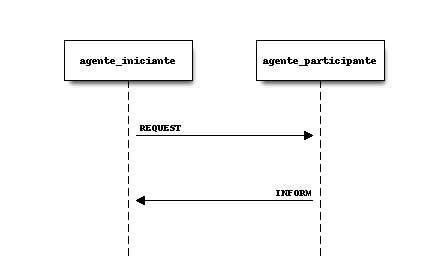
\includegraphics[width=4.5in]{seq_diag_request.png}\hfill}

Para exemplificar o protocolo FIPA-Request, iremos utilizar como exemplo a interação entre dois agentes, um agente relogio, que a cada um segundo exibe na tela a data e o horário atuais, mas com um problema, o agente relogio não sabe calcular nem a data, e muito menos o horário atual. Assim, ele precisa requisitar estas informações do agente horario que consegue calcular estas informações.

Dessa forma, será utilizado o protocolo FIPA-Request, para que estas informações sejam trocadas entre os dois agentes, sendo o agente relógio o iniciante, no processo de requisição e o agente horário, o participante, segue o código do exemplo:

\begin{Verbatim}[commandchars=\\\{\}]
\PYG{k+kn}{from} \PYG{n+nn}{pade.misc.common} \PYG{k+kn}{import} \PYG{n}{start\PYGZus{}loop}\PYG{p}{,} \PYG{n}{set\PYGZus{}ams}
\PYG{k+kn}{from} \PYG{n+nn}{pade.misc.utility} \PYG{k+kn}{import} \PYG{n}{display\PYGZus{}message}
\PYG{k+kn}{from} \PYG{n+nn}{pade.core.agent} \PYG{k+kn}{import} \PYG{n}{Agent}
\PYG{k+kn}{from} \PYG{n+nn}{pade.acl.messages} \PYG{k+kn}{import} \PYG{n}{ACLMessage}
\PYG{k+kn}{from} \PYG{n+nn}{pade.acl.aid} \PYG{k+kn}{import} \PYG{n}{AID}
\PYG{k+kn}{from} \PYG{n+nn}{pade.behaviours.protocols} \PYG{k+kn}{import} \PYG{n}{FipaRequestProtocol}
\PYG{k+kn}{from} \PYG{n+nn}{pade.behaviours.protocols} \PYG{k+kn}{import} \PYG{n}{TimedBehaviour}

\PYG{k+kn}{from} \PYG{n+nn}{datetime} \PYG{k+kn}{import} \PYG{n}{datetime}


\PYG{k}{class} \PYG{n+nc}{CompRequest}\PYG{p}{(}\PYG{n}{FipaRequestProtocol}\PYG{p}{)}\PYG{p}{:}
    \PYG{l+s+sd}{\PYGZdq{}\PYGZdq{}\PYGZdq{}Comportamento FIPA Request}
\PYG{l+s+sd}{    do agente Horario\PYGZdq{}\PYGZdq{}\PYGZdq{}}
    \PYG{k}{def} \PYG{n+nf}{\PYGZus{}\PYGZus{}init\PYGZus{}\PYGZus{}}\PYG{p}{(}\PYG{n+nb+bp}{self}\PYG{p}{,} \PYG{n}{agent}\PYG{p}{)}\PYG{p}{:}
        \PYG{n+nb}{super}\PYG{p}{(}\PYG{n}{CompRequest}\PYG{p}{,} \PYG{n+nb+bp}{self}\PYG{p}{)}\PYG{o}{.}\PYG{n}{\PYGZus{}\PYGZus{}init\PYGZus{}\PYGZus{}}\PYG{p}{(}\PYG{n}{agent}\PYG{o}{=}\PYG{n}{agent}\PYG{p}{,}
                                          \PYG{n}{message}\PYG{o}{=}\PYG{n+nb+bp}{None}\PYG{p}{,}
                                          \PYG{n}{is\PYGZus{}initiator}\PYG{o}{=}\PYG{n+nb+bp}{False}\PYG{p}{)}

    \PYG{k}{def} \PYG{n+nf}{handle\PYGZus{}request}\PYG{p}{(}\PYG{n+nb+bp}{self}\PYG{p}{,} \PYG{n}{message}\PYG{p}{)}\PYG{p}{:}
        \PYG{n+nb}{super}\PYG{p}{(}\PYG{n}{CompRequest}\PYG{p}{,} \PYG{n+nb+bp}{self}\PYG{p}{)}\PYG{o}{.}\PYG{n}{handle\PYGZus{}request}\PYG{p}{(}\PYG{n}{message}\PYG{p}{)}
        \PYG{n}{display\PYGZus{}message}\PYG{p}{(}\PYG{n+nb+bp}{self}\PYG{o}{.}\PYG{n}{agent}\PYG{o}{.}\PYG{n}{aid}\PYG{o}{.}\PYG{n}{localname}\PYG{p}{,} \PYG{l+s}{\PYGZsq{}}\PYG{l+s}{mensagem request recebida}\PYG{l+s}{\PYGZsq{}}\PYG{p}{)}
        \PYG{n}{now} \PYG{o}{=} \PYG{n}{datetime}\PYG{o}{.}\PYG{n}{now}\PYG{p}{(}\PYG{p}{)}
        \PYG{n}{reply} \PYG{o}{=} \PYG{n}{message}\PYG{o}{.}\PYG{n}{create\PYGZus{}reply}\PYG{p}{(}\PYG{p}{)}
        \PYG{n}{reply}\PYG{o}{.}\PYG{n}{set\PYGZus{}performative}\PYG{p}{(}\PYG{n}{ACLMessage}\PYG{o}{.}\PYG{n}{INFORM}\PYG{p}{)}
        \PYG{n}{reply}\PYG{o}{.}\PYG{n}{set\PYGZus{}content}\PYG{p}{(}\PYG{n}{now}\PYG{o}{.}\PYG{n}{strftime}\PYG{p}{(}\PYG{l+s}{\PYGZsq{}}\PYG{l+s+si}{\PYGZpc{}d}\PYG{l+s}{/}\PYG{l+s}{\PYGZpc{}}\PYG{l+s}{m/}\PYG{l+s}{\PYGZpc{}}\PYG{l+s}{Y \PYGZhy{} }\PYG{l+s}{\PYGZpc{}}\PYG{l+s}{H:}\PYG{l+s}{\PYGZpc{}}\PYG{l+s}{M:}\PYG{l+s}{\PYGZpc{}}\PYG{l+s}{S}\PYG{l+s}{\PYGZsq{}}\PYG{p}{)}\PYG{p}{)}
        \PYG{n+nb+bp}{self}\PYG{o}{.}\PYG{n}{agent}\PYG{o}{.}\PYG{n}{send}\PYG{p}{(}\PYG{n}{reply}\PYG{p}{)}


\PYG{k}{class} \PYG{n+nc}{CompRequest2}\PYG{p}{(}\PYG{n}{FipaRequestProtocol}\PYG{p}{)}\PYG{p}{:}
    \PYG{l+s+sd}{\PYGZdq{}\PYGZdq{}\PYGZdq{}Comportamento FIPA Request}
\PYG{l+s+sd}{    do agente Relogio\PYGZdq{}\PYGZdq{}\PYGZdq{}}
    \PYG{k}{def} \PYG{n+nf}{\PYGZus{}\PYGZus{}init\PYGZus{}\PYGZus{}}\PYG{p}{(}\PYG{n+nb+bp}{self}\PYG{p}{,} \PYG{n}{agent}\PYG{p}{,} \PYG{n}{message}\PYG{p}{)}\PYG{p}{:}
        \PYG{n+nb}{super}\PYG{p}{(}\PYG{n}{CompRequest2}\PYG{p}{,} \PYG{n+nb+bp}{self}\PYG{p}{)}\PYG{o}{.}\PYG{n}{\PYGZus{}\PYGZus{}init\PYGZus{}\PYGZus{}}\PYG{p}{(}\PYG{n}{agent}\PYG{o}{=}\PYG{n}{agent}\PYG{p}{,}
                                           \PYG{n}{message}\PYG{o}{=}\PYG{n}{message}\PYG{p}{,}
                                           \PYG{n}{is\PYGZus{}initiator}\PYG{o}{=}\PYG{n+nb+bp}{True}\PYG{p}{)}

    \PYG{k}{def} \PYG{n+nf}{handle\PYGZus{}inform}\PYG{p}{(}\PYG{n+nb+bp}{self}\PYG{p}{,} \PYG{n}{message}\PYG{p}{)}\PYG{p}{:}
        \PYG{n}{display\PYGZus{}message}\PYG{p}{(}\PYG{n+nb+bp}{self}\PYG{o}{.}\PYG{n}{agent}\PYG{o}{.}\PYG{n}{aid}\PYG{o}{.}\PYG{n}{localname}\PYG{p}{,} \PYG{n}{message}\PYG{o}{.}\PYG{n}{content}\PYG{p}{)}


\PYG{k}{class} \PYG{n+nc}{ComportTemporal}\PYG{p}{(}\PYG{n}{TimedBehaviour}\PYG{p}{)}\PYG{p}{:}
    \PYG{l+s+sd}{\PYGZdq{}\PYGZdq{}\PYGZdq{}Comportamento FIPA Request}
\PYG{l+s+sd}{    do agente Relogio\PYGZdq{}\PYGZdq{}\PYGZdq{}}
    \PYG{k}{def} \PYG{n+nf}{\PYGZus{}\PYGZus{}init\PYGZus{}\PYGZus{}}\PYG{p}{(}\PYG{n+nb+bp}{self}\PYG{p}{,} \PYG{n}{agent}\PYG{p}{,} \PYG{n}{time}\PYG{p}{,} \PYG{n}{message}\PYG{p}{)}\PYG{p}{:}
        \PYG{n+nb}{super}\PYG{p}{(}\PYG{n}{ComportTemporal}\PYG{p}{,} \PYG{n+nb+bp}{self}\PYG{p}{)}\PYG{o}{.}\PYG{n}{\PYGZus{}\PYGZus{}init\PYGZus{}\PYGZus{}}\PYG{p}{(}\PYG{n}{agent}\PYG{p}{,} \PYG{n}{time}\PYG{p}{)}
        \PYG{n+nb+bp}{self}\PYG{o}{.}\PYG{n}{message} \PYG{o}{=} \PYG{n}{message}

    \PYG{k}{def} \PYG{n+nf}{on\PYGZus{}time}\PYG{p}{(}\PYG{n+nb+bp}{self}\PYG{p}{)}\PYG{p}{:}
        \PYG{n+nb}{super}\PYG{p}{(}\PYG{n}{ComportTemporal}\PYG{p}{,} \PYG{n+nb+bp}{self}\PYG{p}{)}\PYG{o}{.}\PYG{n}{on\PYGZus{}time}\PYG{p}{(}\PYG{p}{)}
        \PYG{n+nb+bp}{self}\PYG{o}{.}\PYG{n}{agent}\PYG{o}{.}\PYG{n}{send}\PYG{p}{(}\PYG{n+nb+bp}{self}\PYG{o}{.}\PYG{n}{message}\PYG{p}{)}


\PYG{k}{class} \PYG{n+nc}{AgenteHorario}\PYG{p}{(}\PYG{n}{Agent}\PYG{p}{)}\PYG{p}{:}
    \PYG{l+s+sd}{\PYGZdq{}\PYGZdq{}\PYGZdq{}Classe que define o agente Horario\PYGZdq{}\PYGZdq{}\PYGZdq{}}
    \PYG{k}{def} \PYG{n+nf}{\PYGZus{}\PYGZus{}init\PYGZus{}\PYGZus{}}\PYG{p}{(}\PYG{n+nb+bp}{self}\PYG{p}{,} \PYG{n}{aid}\PYG{p}{)}\PYG{p}{:}
        \PYG{n+nb}{super}\PYG{p}{(}\PYG{n}{AgenteHorario}\PYG{p}{,} \PYG{n+nb+bp}{self}\PYG{p}{)}\PYG{o}{.}\PYG{n}{\PYGZus{}\PYGZus{}init\PYGZus{}\PYGZus{}}\PYG{p}{(}\PYG{n}{aid}\PYG{o}{=}\PYG{n}{aid}\PYG{p}{,} \PYG{n}{debug}\PYG{o}{=}\PYG{n+nb+bp}{False}\PYG{p}{)}

        \PYG{n+nb+bp}{self}\PYG{o}{.}\PYG{n}{comport\PYGZus{}request} \PYG{o}{=} \PYG{n}{CompRequest}\PYG{p}{(}\PYG{n+nb+bp}{self}\PYG{p}{)}

        \PYG{n+nb+bp}{self}\PYG{o}{.}\PYG{n}{behaviours}\PYG{o}{.}\PYG{n}{append}\PYG{p}{(}\PYG{n+nb+bp}{self}\PYG{o}{.}\PYG{n}{comport\PYGZus{}request}\PYG{p}{)}


\PYG{k}{class} \PYG{n+nc}{AgenteRelogio}\PYG{p}{(}\PYG{n}{Agent}\PYG{p}{)}\PYG{p}{:}
    \PYG{l+s+sd}{\PYGZdq{}\PYGZdq{}\PYGZdq{}Classe que define o agente Relogio\PYGZdq{}\PYGZdq{}\PYGZdq{}}
    \PYG{k}{def} \PYG{n+nf}{\PYGZus{}\PYGZus{}init\PYGZus{}\PYGZus{}}\PYG{p}{(}\PYG{n+nb+bp}{self}\PYG{p}{,} \PYG{n}{aid}\PYG{p}{)}\PYG{p}{:}
        \PYG{n+nb}{super}\PYG{p}{(}\PYG{n}{AgenteRelogio}\PYG{p}{,} \PYG{n+nb+bp}{self}\PYG{p}{)}\PYG{o}{.}\PYG{n}{\PYGZus{}\PYGZus{}init\PYGZus{}\PYGZus{}}\PYG{p}{(}\PYG{n}{aid}\PYG{o}{=}\PYG{n}{aid}\PYG{p}{)}

        \PYG{c}{\PYGZsh{} mensagem que requisita horario do horario}
        \PYG{n}{message} \PYG{o}{=} \PYG{n}{ACLMessage}\PYG{p}{(}\PYG{n}{ACLMessage}\PYG{o}{.}\PYG{n}{REQUEST}\PYG{p}{)}
        \PYG{n}{message}\PYG{o}{.}\PYG{n}{set\PYGZus{}protocol}\PYG{p}{(}\PYG{n}{ACLMessage}\PYG{o}{.}\PYG{n}{FIPA\PYGZus{}REQUEST\PYGZus{}PROTOCOL}\PYG{p}{)}
        \PYG{n}{message}\PYG{o}{.}\PYG{n}{add\PYGZus{}receiver}\PYG{p}{(}\PYG{n}{AID}\PYG{p}{(}\PYG{n}{name}\PYG{o}{=}\PYG{l+s}{\PYGZsq{}}\PYG{l+s}{horario}\PYG{l+s}{\PYGZsq{}}\PYG{p}{)}\PYG{p}{)}
        \PYG{n}{message}\PYG{o}{.}\PYG{n}{set\PYGZus{}content}\PYG{p}{(}\PYG{l+s}{\PYGZsq{}}\PYG{l+s}{time}\PYG{l+s}{\PYGZsq{}}\PYG{p}{)}

        \PYG{n+nb+bp}{self}\PYG{o}{.}\PYG{n}{comport\PYGZus{}request} \PYG{o}{=} \PYG{n}{CompRequest2}\PYG{p}{(}\PYG{n+nb+bp}{self}\PYG{p}{,} \PYG{n}{message}\PYG{p}{)}
        \PYG{n+nb+bp}{self}\PYG{o}{.}\PYG{n}{comport\PYGZus{}temp} \PYG{o}{=} \PYG{n}{ComportTemporal}\PYG{p}{(}\PYG{n+nb+bp}{self}\PYG{p}{,} \PYG{l+m+mf}{1.0}\PYG{p}{,} \PYG{n}{message}\PYG{p}{)}

        \PYG{n+nb+bp}{self}\PYG{o}{.}\PYG{n}{behaviours}\PYG{o}{.}\PYG{n}{append}\PYG{p}{(}\PYG{n+nb+bp}{self}\PYG{o}{.}\PYG{n}{comport\PYGZus{}request}\PYG{p}{)}
        \PYG{n+nb+bp}{self}\PYG{o}{.}\PYG{n}{behaviours}\PYG{o}{.}\PYG{n}{append}\PYG{p}{(}\PYG{n+nb+bp}{self}\PYG{o}{.}\PYG{n}{comport\PYGZus{}temp}\PYG{p}{)}


\PYG{k}{def} \PYG{n+nf}{main}\PYG{p}{(}\PYG{p}{)}\PYG{p}{:}
    \PYG{n}{agentes} \PYG{o}{=} \PYG{n+nb}{list}\PYG{p}{(}\PYG{p}{)}
    \PYG{n}{set\PYGZus{}ams}\PYG{p}{(}\PYG{l+s}{\PYGZsq{}}\PYG{l+s}{localhost}\PYG{l+s}{\PYGZsq{}}\PYG{p}{,} \PYG{l+m+mi}{8000}\PYG{p}{,} \PYG{n}{debug}\PYG{o}{=}\PYG{n+nb+bp}{False}\PYG{p}{)}

    \PYG{n}{a} \PYG{o}{=} \PYG{n}{AgenteHorario}\PYG{p}{(}\PYG{n}{AID}\PYG{p}{(}\PYG{n}{name}\PYG{o}{=}\PYG{l+s}{\PYGZsq{}}\PYG{l+s}{horario}\PYG{l+s}{\PYGZsq{}}\PYG{p}{)}\PYG{p}{)}
    \PYG{n}{a}\PYG{o}{.}\PYG{n}{ams} \PYG{o}{=} \PYG{p}{\PYGZob{}}\PYG{l+s}{\PYGZsq{}}\PYG{l+s}{name}\PYG{l+s}{\PYGZsq{}}\PYG{p}{:} \PYG{l+s}{\PYGZsq{}}\PYG{l+s}{localhost}\PYG{l+s}{\PYGZsq{}}\PYG{p}{,} \PYG{l+s}{\PYGZsq{}}\PYG{l+s}{port}\PYG{l+s}{\PYGZsq{}}\PYG{p}{:} \PYG{l+m+mi}{8000}\PYG{p}{\PYGZcb{}}
    \PYG{n}{agentes}\PYG{o}{.}\PYG{n}{append}\PYG{p}{(}\PYG{n}{a}\PYG{p}{)}

    \PYG{n}{a} \PYG{o}{=} \PYG{n}{AgenteRelogio}\PYG{p}{(}\PYG{n}{AID}\PYG{p}{(}\PYG{n}{name}\PYG{o}{=}\PYG{l+s}{\PYGZsq{}}\PYG{l+s}{relogio}\PYG{l+s}{\PYGZsq{}}\PYG{p}{)}\PYG{p}{)}
    \PYG{n}{a}\PYG{o}{.}\PYG{n}{ams} \PYG{o}{=} \PYG{p}{\PYGZob{}}\PYG{l+s}{\PYGZsq{}}\PYG{l+s}{name}\PYG{l+s}{\PYGZsq{}}\PYG{p}{:} \PYG{l+s}{\PYGZsq{}}\PYG{l+s}{localhost}\PYG{l+s}{\PYGZsq{}}\PYG{p}{,} \PYG{l+s}{\PYGZsq{}}\PYG{l+s}{port}\PYG{l+s}{\PYGZsq{}}\PYG{p}{:} \PYG{l+m+mi}{8000}\PYG{p}{\PYGZcb{}}
    \PYG{n}{agentes}\PYG{o}{.}\PYG{n}{append}\PYG{p}{(}\PYG{n}{a}\PYG{p}{)}

    \PYG{n}{start\PYGZus{}loop}\PYG{p}{(}\PYG{n}{agentes}\PYG{p}{,} \PYG{n}{gui}\PYG{o}{=}\PYG{n+nb+bp}{True}\PYG{p}{)}

\PYG{k}{if} \PYG{n}{\PYGZus{}\PYGZus{}name\PYGZus{}\PYGZus{}} \PYG{o}{==} \PYG{l+s}{\PYGZsq{}}\PYG{l+s}{\PYGZus{}\PYGZus{}main\PYGZus{}\PYGZus{}}\PYG{l+s}{\PYGZsq{}}\PYG{p}{:}
    \PYG{n}{main}\PYG{p}{(}\PYG{p}{)}
\end{Verbatim}

Na primeira parte do código são importadas todos módulos e classes necessários à construção dos agentes, logo em seguida as classes que implementam o protocolo são definidas, as classes ComptRequest e ComptRequest2 que serão associadas aos comportamentos dos agentes horario e relogio, respectivamente. Como o agente relogio precisa, a cada segundo enviar requisição ao agente horario, então também deve ser associado a este agente um comportamento temporal, definido na classe ComportTemporal que envia uma solicitação ao agente horario, a cada segundo.

Em seguida, os agente propriamente ditos, são definidos nas classes AgenteHoraio e AgenteRelogio que estendem a classe Agent, nessas classes é que os comportamentos e protocolos são associados a cada agente.

Na ultima parte do código, é definida uma função main que indica a localização do agente ams, instancia os agentes e dá inicio ao loop de execução.


\subsection{FIPA-Contract-Net}
\label{user/protocolos:fipa-contract-net}\label{user/protocolos:id2}
O protocolo FIPA-Contract-Net é utilizado para situações onde é necessário realizar algum tipo de negociação entre agentes. Da mesma forma que no protocolo FIPA-Request, no protocolo FIPA-ContractNet existem dois tipos de agentes, um agente que inicia a negociação, ou agente iniciante, fazendo solicitação de propostas e um ou mais agentes que participam da negociação, ou agentes pasticipantes, que repondem às solicitações de propostas do agente iniciante. Veja:
\begin{figure}[htbp]
\centering

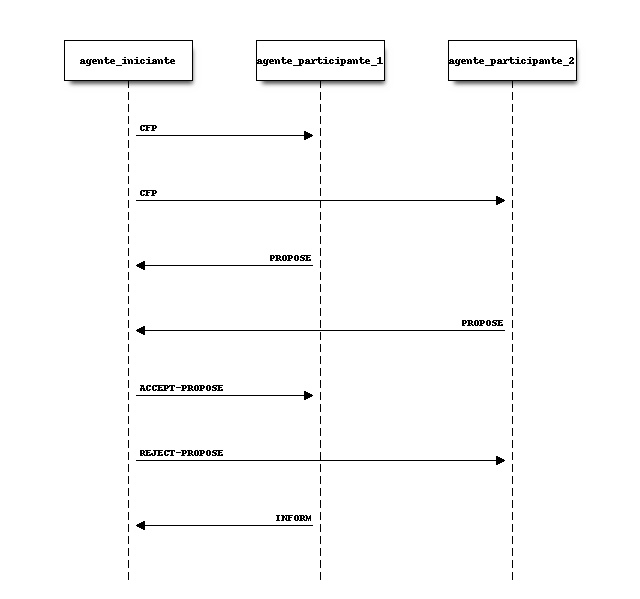
\includegraphics[width=4.5in]{seq_diag_contract.png}
\end{figure}

Um exemplo de utilização do protocolo FIPA-ContractNet na negociação é mostrado abaixo, com a solicitação de um agente iniciante por potência elétrica a outros dois agentes participantes:

\begin{Verbatim}[commandchars=\\\{\}]
\PYG{k+kn}{from} \PYG{n+nn}{pade.misc.common} \PYG{k+kn}{import} \PYG{n}{start\PYGZus{}loop}\PYG{p}{,} \PYG{n}{set\PYGZus{}ams}
\PYG{k+kn}{from} \PYG{n+nn}{pade.misc.utility} \PYG{k+kn}{import} \PYG{n}{display\PYGZus{}message}
\PYG{k+kn}{from} \PYG{n+nn}{pade.core.agent} \PYG{k+kn}{import} \PYG{n}{Agent}
\PYG{k+kn}{from} \PYG{n+nn}{pade.acl.messages} \PYG{k+kn}{import} \PYG{n}{ACLMessage}
\PYG{k+kn}{from} \PYG{n+nn}{pade.acl.aid} \PYG{k+kn}{import} \PYG{n}{AID}
\PYG{k+kn}{from} \PYG{n+nn}{pade.behaviours.protocols} \PYG{k+kn}{import} \PYG{n}{FipaContractNetProtocol}


\PYG{k}{class} \PYG{n+nc}{CompContNet1}\PYG{p}{(}\PYG{n}{FipaContractNetProtocol}\PYG{p}{)}\PYG{p}{:}
    \PYG{l+s+sd}{\PYGZsq{}\PYGZsq{}\PYGZsq{}CompContNet1}

\PYG{l+s+sd}{       Comportamento FIPA\PYGZhy{}ContractNet Iniciante que envia mensagens}
\PYG{l+s+sd}{       CFP para outros agentes alimentadores solicitando propostas}
\PYG{l+s+sd}{       de restauração. Este comportamento também faz a analise das}
\PYG{l+s+sd}{       das propostas e analisa\PYGZhy{}as selecionando a que julga ser a}
\PYG{l+s+sd}{       melhor\PYGZsq{}\PYGZsq{}\PYGZsq{}}

    \PYG{k}{def} \PYG{n+nf}{\PYGZus{}\PYGZus{}init\PYGZus{}\PYGZus{}}\PYG{p}{(}\PYG{n+nb+bp}{self}\PYG{p}{,} \PYG{n}{agent}\PYG{p}{,} \PYG{n}{message}\PYG{p}{)}\PYG{p}{:}
        \PYG{n+nb}{super}\PYG{p}{(}\PYG{n}{CompContNet1}\PYG{p}{,} \PYG{n+nb+bp}{self}\PYG{p}{)}\PYG{o}{.}\PYG{n}{\PYGZus{}\PYGZus{}init\PYGZus{}\PYGZus{}}\PYG{p}{(}
            \PYG{n}{agent}\PYG{o}{=}\PYG{n}{agent}\PYG{p}{,} \PYG{n}{message}\PYG{o}{=}\PYG{n}{message}\PYG{p}{,} \PYG{n}{is\PYGZus{}initiator}\PYG{o}{=}\PYG{n+nb+bp}{True}\PYG{p}{)}
        \PYG{n+nb+bp}{self}\PYG{o}{.}\PYG{n}{cfp} \PYG{o}{=} \PYG{n}{message}

    \PYG{k}{def} \PYG{n+nf}{handle\PYGZus{}all\PYGZus{}proposes}\PYG{p}{(}\PYG{n+nb+bp}{self}\PYG{p}{,} \PYG{n}{proposes}\PYG{p}{)}\PYG{p}{:}
        \PYG{l+s+sd}{\PYGZdq{}\PYGZdq{}\PYGZdq{}}
\PYG{l+s+sd}{        \PYGZdq{}\PYGZdq{}\PYGZdq{}}

        \PYG{n+nb}{super}\PYG{p}{(}\PYG{n}{CompContNet1}\PYG{p}{,} \PYG{n+nb+bp}{self}\PYG{p}{)}\PYG{o}{.}\PYG{n}{handle\PYGZus{}all\PYGZus{}proposes}\PYG{p}{(}\PYG{n}{proposes}\PYG{p}{)}

        \PYG{n}{melhor\PYGZus{}propositor} \PYG{o}{=} \PYG{n+nb+bp}{None}
        \PYG{n}{maior\PYGZus{}potencia} \PYG{o}{=} \PYG{l+m+mf}{0.0}
        \PYG{n}{demais\PYGZus{}propositores} \PYG{o}{=} \PYG{n+nb}{list}\PYG{p}{(}\PYG{p}{)}
        \PYG{n}{display\PYGZus{}message}\PYG{p}{(}\PYG{n+nb+bp}{self}\PYG{o}{.}\PYG{n}{agent}\PYG{o}{.}\PYG{n}{aid}\PYG{o}{.}\PYG{n}{name}\PYG{p}{,} \PYG{l+s}{\PYGZsq{}}\PYG{l+s}{Analisando propostas...}\PYG{l+s}{\PYGZsq{}}\PYG{p}{)}

        \PYG{n}{i} \PYG{o}{=} \PYG{l+m+mi}{1}

        \PYG{c}{\PYGZsh{} lógica de seleção de propostas pela maior potência disponibilizada}
        \PYG{k}{for} \PYG{n}{message} \PYG{o+ow}{in} \PYG{n}{proposes}\PYG{p}{:}
            \PYG{n}{content} \PYG{o}{=} \PYG{n}{message}\PYG{o}{.}\PYG{n}{content}
            \PYG{n}{potencia} \PYG{o}{=} \PYG{n+nb}{float}\PYG{p}{(}\PYG{n}{content}\PYG{p}{)}
            \PYG{n}{display\PYGZus{}message}\PYG{p}{(}\PYG{n+nb+bp}{self}\PYG{o}{.}\PYG{n}{agent}\PYG{o}{.}\PYG{n}{aid}\PYG{o}{.}\PYG{n}{name}\PYG{p}{,}
                            \PYG{l+s}{\PYGZsq{}}\PYG{l+s}{Analisando proposta \PYGZob{}i\PYGZcb{}}\PYG{l+s}{\PYGZsq{}}\PYG{o}{.}\PYG{n}{format}\PYG{p}{(}\PYG{n}{i}\PYG{o}{=}\PYG{n}{i}\PYG{p}{)}\PYG{p}{)}
            \PYG{n}{display\PYGZus{}message}\PYG{p}{(}\PYG{n+nb+bp}{self}\PYG{o}{.}\PYG{n}{agent}\PYG{o}{.}\PYG{n}{aid}\PYG{o}{.}\PYG{n}{name}\PYG{p}{,}
                            \PYG{l+s}{\PYGZsq{}}\PYG{l+s}{Potencia Ofertada: \PYGZob{}pot\PYGZcb{}}\PYG{l+s}{\PYGZsq{}}\PYG{o}{.}\PYG{n}{format}\PYG{p}{(}\PYG{n}{pot}\PYG{o}{=}\PYG{n}{potencia}\PYG{p}{)}\PYG{p}{)}
            \PYG{n}{i} \PYG{o}{+}\PYG{o}{=} \PYG{l+m+mi}{1}
            \PYG{k}{if} \PYG{n}{potencia} \PYG{o}{\PYGZgt{}} \PYG{n}{maior\PYGZus{}potencia}\PYG{p}{:}
                \PYG{k}{if} \PYG{n}{melhor\PYGZus{}propositor} \PYG{o+ow}{is} \PYG{o+ow}{not} \PYG{n+nb+bp}{None}\PYG{p}{:}
                    \PYG{n}{demais\PYGZus{}propositores}\PYG{o}{.}\PYG{n}{append}\PYG{p}{(}\PYG{n}{melhor\PYGZus{}propositor}\PYG{p}{)}

                \PYG{n}{maior\PYGZus{}potencia} \PYG{o}{=} \PYG{n}{potencia}
                \PYG{n}{melhor\PYGZus{}propositor} \PYG{o}{=} \PYG{n}{message}\PYG{o}{.}\PYG{n}{sender}
            \PYG{k}{else}\PYG{p}{:}
                \PYG{n}{demais\PYGZus{}propositores}\PYG{o}{.}\PYG{n}{append}\PYG{p}{(}\PYG{n}{message}\PYG{o}{.}\PYG{n}{sender}\PYG{p}{)}

        \PYG{n}{display\PYGZus{}message}\PYG{p}{(}\PYG{n+nb+bp}{self}\PYG{o}{.}\PYG{n}{agent}\PYG{o}{.}\PYG{n}{aid}\PYG{o}{.}\PYG{n}{name}\PYG{p}{,}
                        \PYG{l+s}{\PYGZsq{}}\PYG{l+s}{A melhor proposta foi de: \PYGZob{}pot\PYGZcb{} VA}\PYG{l+s}{\PYGZsq{}}\PYG{o}{.}\PYG{n}{format}\PYG{p}{(}
                            \PYG{n}{pot}\PYG{o}{=}\PYG{n}{maior\PYGZus{}potencia}\PYG{p}{)}\PYG{p}{)}

        \PYG{k}{if} \PYG{n}{demais\PYGZus{}propositores} \PYG{o}{!=} \PYG{p}{[}\PYG{p}{]}\PYG{p}{:}
            \PYG{n}{display\PYGZus{}message}\PYG{p}{(}\PYG{n+nb+bp}{self}\PYG{o}{.}\PYG{n}{agent}\PYG{o}{.}\PYG{n}{aid}\PYG{o}{.}\PYG{n}{name}\PYG{p}{,}
                            \PYG{l+s}{\PYGZsq{}}\PYG{l+s}{Enviando respostas de recusa...}\PYG{l+s}{\PYGZsq{}}\PYG{p}{)}
            \PYG{n}{resposta} \PYG{o}{=} \PYG{n}{ACLMessage}\PYG{p}{(}\PYG{n}{ACLMessage}\PYG{o}{.}\PYG{n}{REJECT\PYGZus{}PROPOSAL}\PYG{p}{)}
            \PYG{n}{resposta}\PYG{o}{.}\PYG{n}{set\PYGZus{}protocol}\PYG{p}{(}\PYG{n}{ACLMessage}\PYG{o}{.}\PYG{n}{FIPA\PYGZus{}CONTRACT\PYGZus{}NET\PYGZus{}PROTOCOL}\PYG{p}{)}
            \PYG{n}{resposta}\PYG{o}{.}\PYG{n}{set\PYGZus{}content}\PYG{p}{(}\PYG{l+s}{\PYGZsq{}}\PYG{l+s}{\PYGZsq{}}\PYG{p}{)}
            \PYG{k}{for} \PYG{n}{agente} \PYG{o+ow}{in} \PYG{n}{demais\PYGZus{}propositores}\PYG{p}{:}
                \PYG{n}{resposta}\PYG{o}{.}\PYG{n}{add\PYGZus{}receiver}\PYG{p}{(}\PYG{n}{agente}\PYG{p}{)}

            \PYG{n+nb+bp}{self}\PYG{o}{.}\PYG{n}{agent}\PYG{o}{.}\PYG{n}{send}\PYG{p}{(}\PYG{n}{resposta}\PYG{p}{)}

        \PYG{k}{if} \PYG{n}{melhor\PYGZus{}propositor} \PYG{o+ow}{is} \PYG{o+ow}{not} \PYG{n+nb+bp}{None}\PYG{p}{:}
            \PYG{n}{display\PYGZus{}message}\PYG{p}{(}\PYG{n+nb+bp}{self}\PYG{o}{.}\PYG{n}{agent}\PYG{o}{.}\PYG{n}{aid}\PYG{o}{.}\PYG{n}{name}\PYG{p}{,}
                            \PYG{l+s}{\PYGZsq{}}\PYG{l+s}{Enviando resposta de aceitacao...}\PYG{l+s}{\PYGZsq{}}\PYG{p}{)}

            \PYG{n}{resposta} \PYG{o}{=} \PYG{n}{ACLMessage}\PYG{p}{(}\PYG{n}{ACLMessage}\PYG{o}{.}\PYG{n}{ACCEPT\PYGZus{}PROPOSAL}\PYG{p}{)}
            \PYG{n}{resposta}\PYG{o}{.}\PYG{n}{set\PYGZus{}protocol}\PYG{p}{(}\PYG{n}{ACLMessage}\PYG{o}{.}\PYG{n}{FIPA\PYGZus{}CONTRACT\PYGZus{}NET\PYGZus{}PROTOCOL}\PYG{p}{)}
            \PYG{n}{resposta}\PYG{o}{.}\PYG{n}{set\PYGZus{}content}\PYG{p}{(}\PYG{l+s}{\PYGZsq{}}\PYG{l+s}{OK}\PYG{l+s}{\PYGZsq{}}\PYG{p}{)}
            \PYG{n}{resposta}\PYG{o}{.}\PYG{n}{add\PYGZus{}receiver}\PYG{p}{(}\PYG{n}{melhor\PYGZus{}propositor}\PYG{p}{)}
            \PYG{n+nb+bp}{self}\PYG{o}{.}\PYG{n}{agent}\PYG{o}{.}\PYG{n}{send}\PYG{p}{(}\PYG{n}{resposta}\PYG{p}{)}

    \PYG{k}{def} \PYG{n+nf}{handle\PYGZus{}inform}\PYG{p}{(}\PYG{n+nb+bp}{self}\PYG{p}{,} \PYG{n}{message}\PYG{p}{)}\PYG{p}{:}
        \PYG{l+s+sd}{\PYGZdq{}\PYGZdq{}\PYGZdq{}}
\PYG{l+s+sd}{        \PYGZdq{}\PYGZdq{}\PYGZdq{}}
        \PYG{n+nb}{super}\PYG{p}{(}\PYG{n}{CompContNet1}\PYG{p}{,} \PYG{n+nb+bp}{self}\PYG{p}{)}\PYG{o}{.}\PYG{n}{handle\PYGZus{}inform}\PYG{p}{(}\PYG{n}{message}\PYG{p}{)}

        \PYG{n}{display\PYGZus{}message}\PYG{p}{(}\PYG{n+nb+bp}{self}\PYG{o}{.}\PYG{n}{agent}\PYG{o}{.}\PYG{n}{aid}\PYG{o}{.}\PYG{n}{name}\PYG{p}{,} \PYG{l+s}{\PYGZsq{}}\PYG{l+s}{Mensagem INFORM recebida}\PYG{l+s}{\PYGZsq{}}\PYG{p}{)}

    \PYG{k}{def} \PYG{n+nf}{handle\PYGZus{}refuse}\PYG{p}{(}\PYG{n+nb+bp}{self}\PYG{p}{,} \PYG{n}{message}\PYG{p}{)}\PYG{p}{:}
        \PYG{l+s+sd}{\PYGZdq{}\PYGZdq{}\PYGZdq{}}
\PYG{l+s+sd}{        \PYGZdq{}\PYGZdq{}\PYGZdq{}}
        \PYG{n+nb}{super}\PYG{p}{(}\PYG{n}{CompContNet1}\PYG{p}{,} \PYG{n+nb+bp}{self}\PYG{p}{)}\PYG{o}{.}\PYG{n}{handle\PYGZus{}refuse}\PYG{p}{(}\PYG{n}{message}\PYG{p}{)}

        \PYG{n}{display\PYGZus{}message}\PYG{p}{(}\PYG{n+nb+bp}{self}\PYG{o}{.}\PYG{n}{agent}\PYG{o}{.}\PYG{n}{aid}\PYG{o}{.}\PYG{n}{name}\PYG{p}{,} \PYG{l+s}{\PYGZsq{}}\PYG{l+s}{Mensagem REFUSE recebida}\PYG{l+s}{\PYGZsq{}}\PYG{p}{)}

    \PYG{k}{def} \PYG{n+nf}{handle\PYGZus{}propose}\PYG{p}{(}\PYG{n+nb+bp}{self}\PYG{p}{,} \PYG{n}{message}\PYG{p}{)}\PYG{p}{:}
        \PYG{l+s+sd}{\PYGZdq{}\PYGZdq{}\PYGZdq{}}
\PYG{l+s+sd}{        \PYGZdq{}\PYGZdq{}\PYGZdq{}}
        \PYG{n+nb}{super}\PYG{p}{(}\PYG{n}{CompContNet1}\PYG{p}{,} \PYG{n+nb+bp}{self}\PYG{p}{)}\PYG{o}{.}\PYG{n}{handle\PYGZus{}propose}\PYG{p}{(}\PYG{n}{message}\PYG{p}{)}

        \PYG{n}{display\PYGZus{}message}\PYG{p}{(}\PYG{n+nb+bp}{self}\PYG{o}{.}\PYG{n}{agent}\PYG{o}{.}\PYG{n}{aid}\PYG{o}{.}\PYG{n}{name}\PYG{p}{,} \PYG{l+s}{\PYGZsq{}}\PYG{l+s}{Mensagem PROPOSE recebida}\PYG{l+s}{\PYGZsq{}}\PYG{p}{)}


\PYG{k}{class} \PYG{n+nc}{CompContNet2}\PYG{p}{(}\PYG{n}{FipaContractNetProtocol}\PYG{p}{)}\PYG{p}{:}
    \PYG{l+s+sd}{\PYGZsq{}\PYGZsq{}\PYGZsq{}CompContNet2}

\PYG{l+s+sd}{       Comportamento FIPA\PYGZhy{}ContractNet Participante que é acionado}
\PYG{l+s+sd}{       quando um agente recebe uma mensagem do Tipo CFP enviando logo}
\PYG{l+s+sd}{       em seguida uma proposta e caso esta seja selecinada realiza as}
\PYG{l+s+sd}{       as análises de restrição para que seja possível a restauração\PYGZsq{}\PYGZsq{}\PYGZsq{}}

    \PYG{k}{def} \PYG{n+nf}{\PYGZus{}\PYGZus{}init\PYGZus{}\PYGZus{}}\PYG{p}{(}\PYG{n+nb+bp}{self}\PYG{p}{,} \PYG{n}{agent}\PYG{p}{)}\PYG{p}{:}
        \PYG{n+nb}{super}\PYG{p}{(}\PYG{n}{CompContNet2}\PYG{p}{,} \PYG{n+nb+bp}{self}\PYG{p}{)}\PYG{o}{.}\PYG{n}{\PYGZus{}\PYGZus{}init\PYGZus{}\PYGZus{}}\PYG{p}{(}\PYG{n}{agent}\PYG{o}{=}\PYG{n}{agent}\PYG{p}{,}
                                           \PYG{n}{message}\PYG{o}{=}\PYG{n+nb+bp}{None}\PYG{p}{,}
                                           \PYG{n}{is\PYGZus{}initiator}\PYG{o}{=}\PYG{n+nb+bp}{False}\PYG{p}{)}

    \PYG{k}{def} \PYG{n+nf}{handle\PYGZus{}cfp}\PYG{p}{(}\PYG{n+nb+bp}{self}\PYG{p}{,} \PYG{n}{message}\PYG{p}{)}\PYG{p}{:}
        \PYG{l+s+sd}{\PYGZdq{}\PYGZdq{}\PYGZdq{}}
\PYG{l+s+sd}{        \PYGZdq{}\PYGZdq{}\PYGZdq{}}
        \PYG{n+nb+bp}{self}\PYG{o}{.}\PYG{n}{agent}\PYG{o}{.}\PYG{n}{call\PYGZus{}later}\PYG{p}{(}\PYG{l+m+mf}{1.0}\PYG{p}{,} \PYG{n+nb+bp}{self}\PYG{o}{.}\PYG{n}{\PYGZus{}handle\PYGZus{}cfp}\PYG{p}{,} \PYG{n}{message}\PYG{p}{)}

    \PYG{k}{def} \PYG{n+nf}{\PYGZus{}handle\PYGZus{}cfp}\PYG{p}{(}\PYG{n+nb+bp}{self}\PYG{p}{,} \PYG{n}{message}\PYG{p}{)}\PYG{p}{:}
        \PYG{l+s+sd}{\PYGZdq{}\PYGZdq{}\PYGZdq{}}
\PYG{l+s+sd}{        \PYGZdq{}\PYGZdq{}\PYGZdq{}}
        \PYG{n+nb}{super}\PYG{p}{(}\PYG{n}{CompContNet2}\PYG{p}{,} \PYG{n+nb+bp}{self}\PYG{p}{)}\PYG{o}{.}\PYG{n}{handle\PYGZus{}cfp}\PYG{p}{(}\PYG{n}{message}\PYG{p}{)}
        \PYG{n+nb+bp}{self}\PYG{o}{.}\PYG{n}{message} \PYG{o}{=} \PYG{n}{message}

        \PYG{n}{display\PYGZus{}message}\PYG{p}{(}\PYG{n+nb+bp}{self}\PYG{o}{.}\PYG{n}{agent}\PYG{o}{.}\PYG{n}{aid}\PYG{o}{.}\PYG{n}{name}\PYG{p}{,} \PYG{l+s}{\PYGZsq{}}\PYG{l+s}{Mensagem CFP recebida}\PYG{l+s}{\PYGZsq{}}\PYG{p}{)}

        \PYG{n}{resposta} \PYG{o}{=} \PYG{n+nb+bp}{self}\PYG{o}{.}\PYG{n}{message}\PYG{o}{.}\PYG{n}{create\PYGZus{}reply}\PYG{p}{(}\PYG{p}{)}
        \PYG{n}{resposta}\PYG{o}{.}\PYG{n}{set\PYGZus{}performative}\PYG{p}{(}\PYG{n}{ACLMessage}\PYG{o}{.}\PYG{n}{PROPOSE}\PYG{p}{)}
        \PYG{n}{resposta}\PYG{o}{.}\PYG{n}{set\PYGZus{}content}\PYG{p}{(}\PYG{n+nb}{str}\PYG{p}{(}\PYG{n+nb+bp}{self}\PYG{o}{.}\PYG{n}{agent}\PYG{o}{.}\PYG{n}{pot\PYGZus{}disp}\PYG{p}{)}\PYG{p}{)}
        \PYG{n+nb+bp}{self}\PYG{o}{.}\PYG{n}{agent}\PYG{o}{.}\PYG{n}{send}\PYG{p}{(}\PYG{n}{resposta}\PYG{p}{)}

    \PYG{k}{def} \PYG{n+nf}{handle\PYGZus{}reject\PYGZus{}propose}\PYG{p}{(}\PYG{n+nb+bp}{self}\PYG{p}{,} \PYG{n}{message}\PYG{p}{)}\PYG{p}{:}
        \PYG{l+s+sd}{\PYGZdq{}\PYGZdq{}\PYGZdq{}}
\PYG{l+s+sd}{        \PYGZdq{}\PYGZdq{}\PYGZdq{}}
        \PYG{n+nb}{super}\PYG{p}{(}\PYG{n}{CompContNet2}\PYG{p}{,} \PYG{n+nb+bp}{self}\PYG{p}{)}\PYG{o}{.}\PYG{n}{handle\PYGZus{}reject\PYGZus{}propose}\PYG{p}{(}\PYG{n}{message}\PYG{p}{)}

        \PYG{n}{display\PYGZus{}message}\PYG{p}{(}\PYG{n+nb+bp}{self}\PYG{o}{.}\PYG{n}{agent}\PYG{o}{.}\PYG{n}{aid}\PYG{o}{.}\PYG{n}{name}\PYG{p}{,}
                        \PYG{l+s}{\PYGZsq{}}\PYG{l+s}{Mensagem REJECT\PYGZus{}PROPOSAL recebida}\PYG{l+s}{\PYGZsq{}}\PYG{p}{)}

    \PYG{k}{def} \PYG{n+nf}{handle\PYGZus{}accept\PYGZus{}propose}\PYG{p}{(}\PYG{n+nb+bp}{self}\PYG{p}{,} \PYG{n}{message}\PYG{p}{)}\PYG{p}{:}
        \PYG{l+s+sd}{\PYGZdq{}\PYGZdq{}\PYGZdq{}}
\PYG{l+s+sd}{        \PYGZdq{}\PYGZdq{}\PYGZdq{}}
        \PYG{n+nb}{super}\PYG{p}{(}\PYG{n}{CompContNet2}\PYG{p}{,} \PYG{n+nb+bp}{self}\PYG{p}{)}\PYG{o}{.}\PYG{n}{handle\PYGZus{}accept\PYGZus{}propose}\PYG{p}{(}\PYG{n}{message}\PYG{p}{)}

        \PYG{n}{display\PYGZus{}message}\PYG{p}{(}\PYG{n+nb+bp}{self}\PYG{o}{.}\PYG{n}{agent}\PYG{o}{.}\PYG{n}{aid}\PYG{o}{.}\PYG{n}{name}\PYG{p}{,}
                        \PYG{l+s}{\PYGZsq{}}\PYG{l+s}{Mensagem ACCEPT\PYGZus{}PROPOSE recebida}\PYG{l+s}{\PYGZsq{}}\PYG{p}{)}

        \PYG{n}{resposta} \PYG{o}{=} \PYG{n}{message}\PYG{o}{.}\PYG{n}{create\PYGZus{}reply}\PYG{p}{(}\PYG{p}{)}
        \PYG{n}{resposta}\PYG{o}{.}\PYG{n}{set\PYGZus{}performative}\PYG{p}{(}\PYG{n}{ACLMessage}\PYG{o}{.}\PYG{n}{INFORM}\PYG{p}{)}
        \PYG{n}{resposta}\PYG{o}{.}\PYG{n}{set\PYGZus{}content}\PYG{p}{(}\PYG{l+s}{\PYGZsq{}}\PYG{l+s}{OK}\PYG{l+s}{\PYGZsq{}}\PYG{p}{)}
        \PYG{n+nb+bp}{self}\PYG{o}{.}\PYG{n}{agent}\PYG{o}{.}\PYG{n}{send}\PYG{p}{(}\PYG{n}{resposta}\PYG{p}{)}


\PYG{k}{class} \PYG{n+nc}{AgenteIniciante}\PYG{p}{(}\PYG{n}{Agent}\PYG{p}{)}\PYG{p}{:}

    \PYG{k}{def} \PYG{n+nf}{\PYGZus{}\PYGZus{}init\PYGZus{}\PYGZus{}}\PYG{p}{(}\PYG{n+nb+bp}{self}\PYG{p}{,} \PYG{n}{aid}\PYG{p}{)}\PYG{p}{:}
        \PYG{n+nb}{super}\PYG{p}{(}\PYG{n}{AgenteIniciante}\PYG{p}{,} \PYG{n+nb+bp}{self}\PYG{p}{)}\PYG{o}{.}\PYG{n}{\PYGZus{}\PYGZus{}init\PYGZus{}\PYGZus{}}\PYG{p}{(}\PYG{n}{aid}\PYG{o}{=}\PYG{n}{aid}\PYG{p}{,} \PYG{n}{debug}\PYG{o}{=}\PYG{n+nb+bp}{False}\PYG{p}{)}

        \PYG{n}{message} \PYG{o}{=} \PYG{n}{ACLMessage}\PYG{p}{(}\PYG{n}{ACLMessage}\PYG{o}{.}\PYG{n}{CFP}\PYG{p}{)}
        \PYG{n}{message}\PYG{o}{.}\PYG{n}{set\PYGZus{}protocol}\PYG{p}{(}\PYG{n}{ACLMessage}\PYG{o}{.}\PYG{n}{FIPA\PYGZus{}CONTRACT\PYGZus{}NET\PYGZus{}PROTOCOL}\PYG{p}{)}
        \PYG{n}{message}\PYG{o}{.}\PYG{n}{set\PYGZus{}content}\PYG{p}{(}\PYG{l+s}{\PYGZsq{}}\PYG{l+s}{60.0}\PYG{l+s}{\PYGZsq{}}\PYG{p}{)}
        \PYG{n}{message}\PYG{o}{.}\PYG{n}{add\PYGZus{}receiver}\PYG{p}{(}\PYG{n}{AID}\PYG{p}{(}\PYG{l+s}{\PYGZsq{}}\PYG{l+s}{AP1}\PYG{l+s}{\PYGZsq{}}\PYG{p}{)}\PYG{p}{)}
        \PYG{n}{message}\PYG{o}{.}\PYG{n}{add\PYGZus{}receiver}\PYG{p}{(}\PYG{n}{AID}\PYG{p}{(}\PYG{l+s}{\PYGZsq{}}\PYG{l+s}{AP2}\PYG{l+s}{\PYGZsq{}}\PYG{p}{)}\PYG{p}{)}

        \PYG{n}{comp} \PYG{o}{=} \PYG{n}{CompContNet1}\PYG{p}{(}\PYG{n+nb+bp}{self}\PYG{p}{,} \PYG{n}{message}\PYG{p}{)}
        \PYG{n+nb+bp}{self}\PYG{o}{.}\PYG{n}{behaviours}\PYG{o}{.}\PYG{n}{append}\PYG{p}{(}\PYG{n}{comp}\PYG{p}{)}
        \PYG{n+nb+bp}{self}\PYG{o}{.}\PYG{n}{call\PYGZus{}later}\PYG{p}{(}\PYG{l+m+mf}{2.0}\PYG{p}{,} \PYG{n}{comp}\PYG{o}{.}\PYG{n}{on\PYGZus{}start}\PYG{p}{)}


\PYG{k}{class} \PYG{n+nc}{AgenteParticipante}\PYG{p}{(}\PYG{n}{Agent}\PYG{p}{)}\PYG{p}{:}

    \PYG{k}{def} \PYG{n+nf}{\PYGZus{}\PYGZus{}init\PYGZus{}\PYGZus{}}\PYG{p}{(}\PYG{n+nb+bp}{self}\PYG{p}{,} \PYG{n}{aid}\PYG{p}{,} \PYG{n}{pot\PYGZus{}disp}\PYG{p}{)}\PYG{p}{:}
        \PYG{n+nb}{super}\PYG{p}{(}\PYG{n}{AgenteParticipante}\PYG{p}{,} \PYG{n+nb+bp}{self}\PYG{p}{)}\PYG{o}{.}\PYG{n}{\PYGZus{}\PYGZus{}init\PYGZus{}\PYGZus{}}\PYG{p}{(}\PYG{n}{aid}\PYG{o}{=}\PYG{n}{aid}\PYG{p}{,} \PYG{n}{debug}\PYG{o}{=}\PYG{n+nb+bp}{False}\PYG{p}{)}

        \PYG{n+nb+bp}{self}\PYG{o}{.}\PYG{n}{pot\PYGZus{}disp} \PYG{o}{=} \PYG{n}{pot\PYGZus{}disp}

        \PYG{n}{comp} \PYG{o}{=} \PYG{n}{CompContNet2}\PYG{p}{(}\PYG{n+nb+bp}{self}\PYG{p}{)}

        \PYG{n+nb+bp}{self}\PYG{o}{.}\PYG{n}{behaviours}\PYG{o}{.}\PYG{n}{append}\PYG{p}{(}\PYG{n}{comp}\PYG{p}{)}

\PYG{k}{if} \PYG{n}{\PYGZus{}\PYGZus{}name\PYGZus{}\PYGZus{}} \PYG{o}{==} \PYG{l+s}{\PYGZdq{}}\PYG{l+s}{\PYGZus{}\PYGZus{}main\PYGZus{}\PYGZus{}}\PYG{l+s}{\PYGZdq{}}\PYG{p}{:}

    \PYG{n}{set\PYGZus{}ams}\PYG{p}{(}\PYG{l+s}{\PYGZsq{}}\PYG{l+s}{localhost}\PYG{l+s}{\PYGZsq{}}\PYG{p}{,} \PYG{l+m+mi}{5000}\PYG{p}{,} \PYG{n}{debug}\PYG{o}{=}\PYG{n+nb+bp}{False}\PYG{p}{)}

    \PYG{n}{aa\PYGZus{}1} \PYG{o}{=} \PYG{n}{AgenteIniciante}\PYG{p}{(}\PYG{n}{AID}\PYG{p}{(}\PYG{n}{name}\PYG{o}{=}\PYG{l+s}{\PYGZsq{}}\PYG{l+s}{AI1}\PYG{l+s}{\PYGZsq{}}\PYG{p}{)}\PYG{p}{)}
    \PYG{n}{aa\PYGZus{}1}\PYG{o}{.}\PYG{n}{ams} \PYG{o}{=} \PYG{p}{\PYGZob{}}\PYG{l+s}{\PYGZsq{}}\PYG{l+s}{name}\PYG{l+s}{\PYGZsq{}}\PYG{p}{:} \PYG{l+s}{\PYGZsq{}}\PYG{l+s}{localhost}\PYG{l+s}{\PYGZsq{}}\PYG{p}{,} \PYG{l+s}{\PYGZsq{}}\PYG{l+s}{port}\PYG{l+s}{\PYGZsq{}}\PYG{p}{:} \PYG{l+m+mi}{5000}\PYG{p}{\PYGZcb{}}

    \PYG{n}{aa\PYGZus{}2} \PYG{o}{=} \PYG{n}{AgenteParticipante}\PYG{p}{(}\PYG{n}{AID}\PYG{p}{(}\PYG{n}{name}\PYG{o}{=}\PYG{l+s}{\PYGZsq{}}\PYG{l+s}{AP1}\PYG{l+s}{\PYGZsq{}}\PYG{p}{)}\PYG{p}{,} \PYG{l+m+mf}{150.0}\PYG{p}{)}
    \PYG{n}{aa\PYGZus{}2}\PYG{o}{.}\PYG{n}{ams} \PYG{o}{=} \PYG{p}{\PYGZob{}}\PYG{l+s}{\PYGZsq{}}\PYG{l+s}{name}\PYG{l+s}{\PYGZsq{}}\PYG{p}{:} \PYG{l+s}{\PYGZsq{}}\PYG{l+s}{localhost}\PYG{l+s}{\PYGZsq{}}\PYG{p}{,} \PYG{l+s}{\PYGZsq{}}\PYG{l+s}{port}\PYG{l+s}{\PYGZsq{}}\PYG{p}{:} \PYG{l+m+mi}{5000}\PYG{p}{\PYGZcb{}}

    \PYG{n}{aa\PYGZus{}3} \PYG{o}{=} \PYG{n}{AgenteParticipante}\PYG{p}{(}\PYG{n}{AID}\PYG{p}{(}\PYG{n}{name}\PYG{o}{=}\PYG{l+s}{\PYGZsq{}}\PYG{l+s}{AP2}\PYG{l+s}{\PYGZsq{}}\PYG{p}{)}\PYG{p}{,} \PYG{l+m+mf}{100.0}\PYG{p}{)}
    \PYG{n}{aa\PYGZus{}3}\PYG{o}{.}\PYG{n}{ams} \PYG{o}{=} \PYG{p}{\PYGZob{}}\PYG{l+s}{\PYGZsq{}}\PYG{l+s}{name}\PYG{l+s}{\PYGZsq{}}\PYG{p}{:} \PYG{l+s}{\PYGZsq{}}\PYG{l+s}{localhost}\PYG{l+s}{\PYGZsq{}}\PYG{p}{,} \PYG{l+s}{\PYGZsq{}}\PYG{l+s}{port}\PYG{l+s}{\PYGZsq{}}\PYG{p}{:} \PYG{l+m+mi}{5000}\PYG{p}{\PYGZcb{}}

    \PYG{n}{agents\PYGZus{}list} \PYG{o}{=} \PYG{n+nb}{list}\PYG{p}{(}\PYG{p}{[}\PYG{n}{aa\PYGZus{}1}\PYG{p}{,} \PYG{n}{aa\PYGZus{}2}\PYG{p}{,} \PYG{n}{aa\PYGZus{}3}\PYG{p}{]}\PYG{p}{)}

    \PYG{n}{start\PYGZus{}loop}\PYG{p}{(}\PYG{n}{agents\PYGZus{}list}\PYG{p}{,} \PYG{n}{gui}\PYG{o}{=}\PYG{n+nb+bp}{True}\PYG{p}{)}
\end{Verbatim}

O código que implementa os agentes que se comunicam utilizando o protocolo FIPA-ContractNet, definine as duas classes do protocolo, a primeira implementa o comportamento do agente Iniciante (CompContNet1) e a segunda implementa o comportamento do agente participante (CompContNet2). Note que para a classe iniciante é necessário que uma mensagem do tipo CFP (call for proposes) seja montada e o método on\_start() seja chamado, isso é feito dentro da classe que implementa os agente iniciante, AgenteIniciante(), já a classe AgenteParticipante(), implementa os agentes que participarão da negociação como propositores.

É possível observar as mensagens da negociação na intergace gráfica do PADE, veja:

{\hfill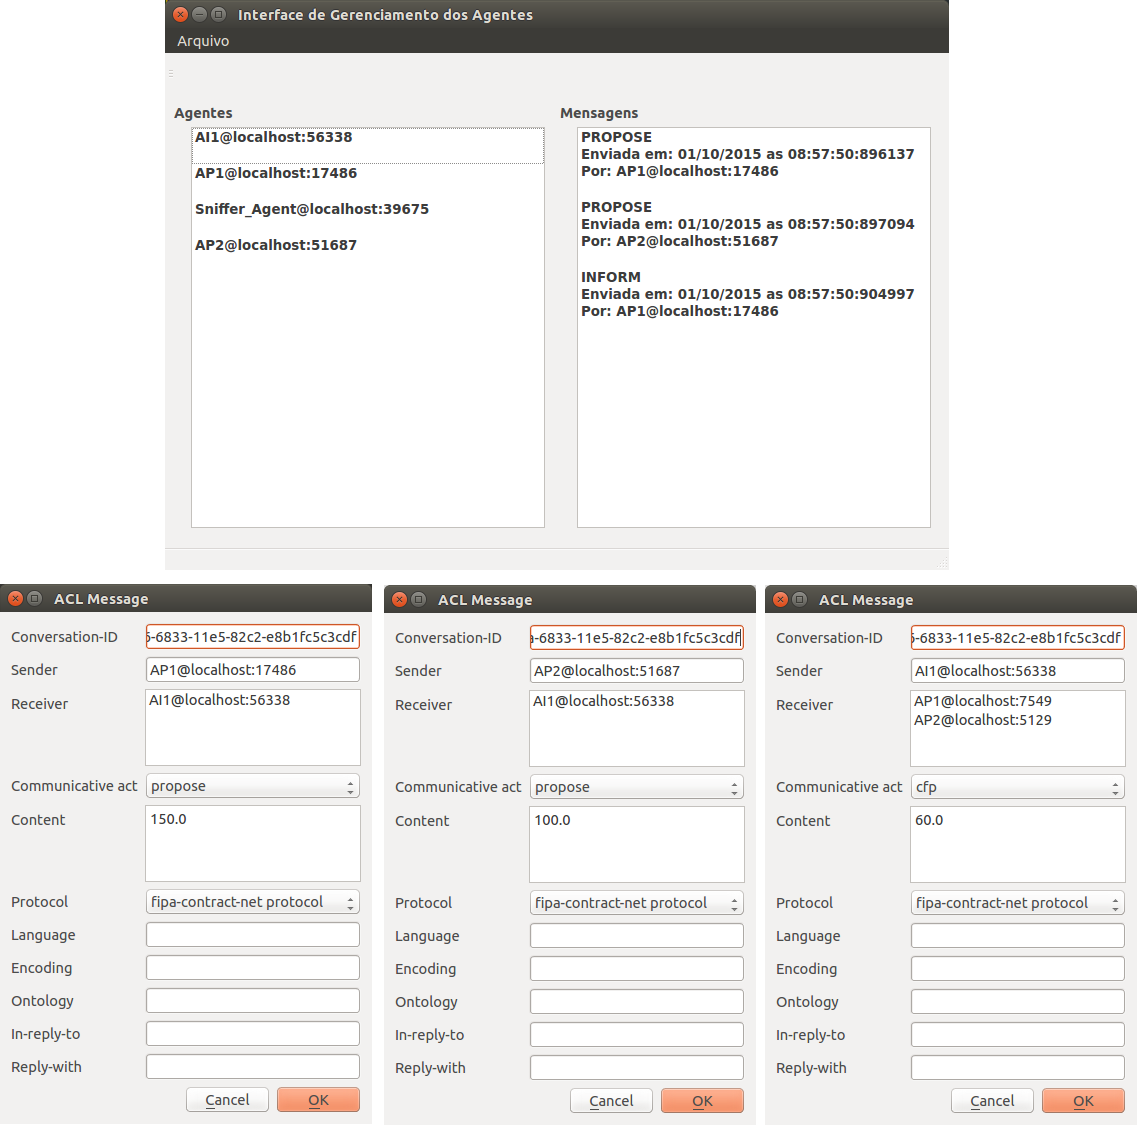
\includegraphics[width=4.5in]{ACLMessage_todas.png}\hfill}


\subsection{FIPA-Subscribe}
\label{user/protocolos:fipa-subscribe}\label{user/protocolos:id3}
O protocolo FIPA-Subscribe, implementa o comportamento de editor-assinante, que conssiste na presença de um agente editor que pode aceitar a associação de outros agentes interessados, agentes assinantes, em algum tipo de informação que este agente possua, assinando a informação e recebendo mensagem sempre que esta informação for disponibilizada pelo agente editor. Veja:
\begin{figure}[htbp]
\centering

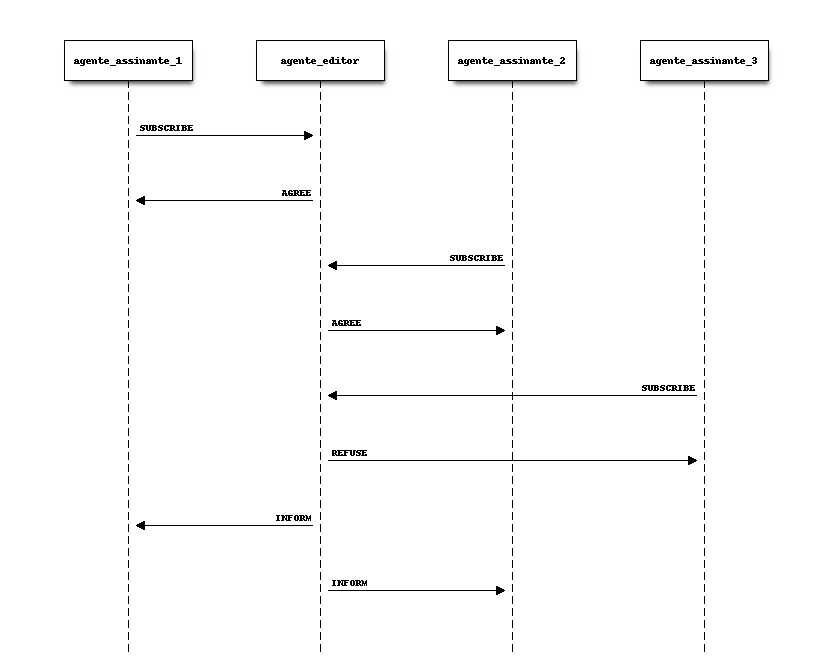
\includegraphics[width=4.5in]{seq_diag_subscribe.png}
\end{figure}

Para assinar a informação o agente precisa enviar uma mensagem SUSBCRIBE para o agente editor. Que por sua vez pode aceitar ou recusar a assinatura (AGREE/REFUSE). Quando uma informação é atualizada, então o editor publica esta informação para todos os seus assinantes, enviando-os mensagens INFORM.

O código que implementa um agente editor e dois agentes assinantes utilizando PADE pode ser visualizado abaixo:

\begin{Verbatim}[commandchars=\\\{\}]
\PYG{k+kn}{from} \PYG{n+nn}{pade.misc.common} \PYG{k+kn}{import} \PYG{n}{start\PYGZus{}loop}\PYG{p}{,} \PYG{n}{set\PYGZus{}ams}
\PYG{k+kn}{from} \PYG{n+nn}{pade.misc.utility} \PYG{k+kn}{import} \PYG{n}{display\PYGZus{}message}
\PYG{k+kn}{from} \PYG{n+nn}{pade.core.agent} \PYG{k+kn}{import} \PYG{n}{Agent}
\PYG{k+kn}{from} \PYG{n+nn}{pade.acl.aid} \PYG{k+kn}{import} \PYG{n}{AID}
\PYG{k+kn}{from} \PYG{n+nn}{pade.acl.messages} \PYG{k+kn}{import} \PYG{n}{ACLMessage}
\PYG{k+kn}{from} \PYG{n+nn}{pade.behaviours.protocols} \PYG{k+kn}{import} \PYG{n}{FipaSubscribeProtocol}\PYG{p}{,} \PYG{n}{TimedBehaviour}
\PYG{k+kn}{from} \PYG{n+nn}{numpy} \PYG{k+kn}{import} \PYG{n}{sin}


\PYG{k}{class} \PYG{n+nc}{SubscribeInitiator}\PYG{p}{(}\PYG{n}{FipaSubscribeProtocol}\PYG{p}{)}\PYG{p}{:}

    \PYG{k}{def} \PYG{n+nf}{\PYGZus{}\PYGZus{}init\PYGZus{}\PYGZus{}}\PYG{p}{(}\PYG{n+nb+bp}{self}\PYG{p}{,} \PYG{n}{agent}\PYG{p}{,} \PYG{n}{message}\PYG{p}{)}\PYG{p}{:}
        \PYG{n+nb}{super}\PYG{p}{(}\PYG{n}{SubscribeInitiator}\PYG{p}{,} \PYG{n+nb+bp}{self}\PYG{p}{)}\PYG{o}{.}\PYG{n}{\PYGZus{}\PYGZus{}init\PYGZus{}\PYGZus{}}\PYG{p}{(}\PYG{n}{agent}\PYG{p}{,}
                                                 \PYG{n}{message}\PYG{p}{,}
                                                 \PYG{n}{is\PYGZus{}initiator}\PYG{o}{=}\PYG{n+nb+bp}{True}\PYG{p}{)}

    \PYG{k}{def} \PYG{n+nf}{handle\PYGZus{}agree}\PYG{p}{(}\PYG{n+nb+bp}{self}\PYG{p}{,} \PYG{n}{message}\PYG{p}{)}\PYG{p}{:}
        \PYG{n}{display\PYGZus{}message}\PYG{p}{(}\PYG{n+nb+bp}{self}\PYG{o}{.}\PYG{n}{agent}\PYG{o}{.}\PYG{n}{aid}\PYG{o}{.}\PYG{n}{name}\PYG{p}{,} \PYG{n}{message}\PYG{o}{.}\PYG{n}{content}\PYG{p}{)}

    \PYG{k}{def} \PYG{n+nf}{handle\PYGZus{}inform}\PYG{p}{(}\PYG{n+nb+bp}{self}\PYG{p}{,} \PYG{n}{message}\PYG{p}{)}\PYG{p}{:}
        \PYG{n}{display\PYGZus{}message}\PYG{p}{(}\PYG{n+nb+bp}{self}\PYG{o}{.}\PYG{n}{agent}\PYG{o}{.}\PYG{n}{aid}\PYG{o}{.}\PYG{n}{name}\PYG{p}{,} \PYG{n}{message}\PYG{o}{.}\PYG{n}{content}\PYG{p}{)}


\PYG{k}{class} \PYG{n+nc}{SubscribeParticipant}\PYG{p}{(}\PYG{n}{FipaSubscribeProtocol}\PYG{p}{)}\PYG{p}{:}

    \PYG{k}{def} \PYG{n+nf}{\PYGZus{}\PYGZus{}init\PYGZus{}\PYGZus{}}\PYG{p}{(}\PYG{n+nb+bp}{self}\PYG{p}{,} \PYG{n}{agent}\PYG{p}{)}\PYG{p}{:}
        \PYG{n+nb}{super}\PYG{p}{(}\PYG{n}{SubscribeParticipant}\PYG{p}{,} \PYG{n+nb+bp}{self}\PYG{p}{)}\PYG{o}{.}\PYG{n}{\PYGZus{}\PYGZus{}init\PYGZus{}\PYGZus{}}\PYG{p}{(}\PYG{n}{agent}\PYG{p}{,}
                                                   \PYG{n}{message}\PYG{o}{=}\PYG{n+nb+bp}{None}\PYG{p}{,}
                                                   \PYG{n}{is\PYGZus{}initiator}\PYG{o}{=}\PYG{n+nb+bp}{False}\PYG{p}{)}

    \PYG{k}{def} \PYG{n+nf}{handle\PYGZus{}subscribe}\PYG{p}{(}\PYG{n+nb+bp}{self}\PYG{p}{,} \PYG{n}{message}\PYG{p}{)}\PYG{p}{:}
        \PYG{n+nb+bp}{self}\PYG{o}{.}\PYG{n}{register}\PYG{p}{(}\PYG{n}{message}\PYG{o}{.}\PYG{n}{sender}\PYG{p}{)}
        \PYG{n}{display\PYGZus{}message}\PYG{p}{(}\PYG{n+nb+bp}{self}\PYG{o}{.}\PYG{n}{agent}\PYG{o}{.}\PYG{n}{aid}\PYG{o}{.}\PYG{n}{name}\PYG{p}{,} \PYG{n}{message}\PYG{o}{.}\PYG{n}{content}\PYG{p}{)}

        \PYG{n}{resposta} \PYG{o}{=} \PYG{n}{message}\PYG{o}{.}\PYG{n}{create\PYGZus{}reply}\PYG{p}{(}\PYG{p}{)}
        \PYG{n}{resposta}\PYG{o}{.}\PYG{n}{set\PYGZus{}performative}\PYG{p}{(}\PYG{n}{ACLMessage}\PYG{o}{.}\PYG{n}{AGREE}\PYG{p}{)}
        \PYG{n}{resposta}\PYG{o}{.}\PYG{n}{set\PYGZus{}content}\PYG{p}{(}\PYG{l+s}{\PYGZsq{}}\PYG{l+s}{Pedido de subscricao aceito}\PYG{l+s}{\PYGZsq{}}\PYG{p}{)}
        \PYG{n+nb+bp}{self}\PYG{o}{.}\PYG{n}{agent}\PYG{o}{.}\PYG{n}{send}\PYG{p}{(}\PYG{n}{resposta}\PYG{p}{)}

    \PYG{k}{def} \PYG{n+nf}{handle\PYGZus{}cancel}\PYG{p}{(}\PYG{n+nb+bp}{self}\PYG{p}{,} \PYG{n}{message}\PYG{p}{)}\PYG{p}{:}
        \PYG{n+nb+bp}{self}\PYG{o}{.}\PYG{n}{deregister}\PYG{p}{(}\PYG{n+nb+bp}{self}\PYG{p}{,} \PYG{n}{message}\PYG{o}{.}\PYG{n}{sender}\PYG{p}{)}
        \PYG{n}{display\PYGZus{}message}\PYG{p}{(}\PYG{n+nb+bp}{self}\PYG{o}{.}\PYG{n}{agent}\PYG{o}{.}\PYG{n}{aid}\PYG{o}{.}\PYG{n}{name}\PYG{p}{,} \PYG{n}{message}\PYG{o}{.}\PYG{n}{content}\PYG{p}{)}

    \PYG{k}{def} \PYG{n+nf}{notify}\PYG{p}{(}\PYG{n+nb+bp}{self}\PYG{p}{,} \PYG{n}{message}\PYG{p}{)}\PYG{p}{:}
        \PYG{n+nb}{super}\PYG{p}{(}\PYG{n}{SubscribeParticipant}\PYG{p}{,} \PYG{n+nb+bp}{self}\PYG{p}{)}\PYG{o}{.}\PYG{n}{notify}\PYG{p}{(}\PYG{n}{message}\PYG{p}{)}


\PYG{k}{class} \PYG{n+nc}{Time}\PYG{p}{(}\PYG{n}{TimedBehaviour}\PYG{p}{)}\PYG{p}{:}

    \PYG{k}{def} \PYG{n+nf}{\PYGZus{}\PYGZus{}init\PYGZus{}\PYGZus{}}\PYG{p}{(}\PYG{n+nb+bp}{self}\PYG{p}{,} \PYG{n}{agent}\PYG{p}{,} \PYG{n}{notify}\PYG{p}{)}\PYG{p}{:}
        \PYG{n+nb}{super}\PYG{p}{(}\PYG{n}{Time}\PYG{p}{,} \PYG{n+nb+bp}{self}\PYG{p}{)}\PYG{o}{.}\PYG{n}{\PYGZus{}\PYGZus{}init\PYGZus{}\PYGZus{}}\PYG{p}{(}\PYG{n}{agent}\PYG{p}{,} \PYG{l+m+mi}{1}\PYG{p}{)}
        \PYG{n+nb+bp}{self}\PYG{o}{.}\PYG{n}{notify} \PYG{o}{=} \PYG{n}{notify}
        \PYG{n+nb+bp}{self}\PYG{o}{.}\PYG{n}{inc} \PYG{o}{=} \PYG{l+m+mi}{0}

    \PYG{k}{def} \PYG{n+nf}{on\PYGZus{}time}\PYG{p}{(}\PYG{n+nb+bp}{self}\PYG{p}{)}\PYG{p}{:}
        \PYG{n+nb}{super}\PYG{p}{(}\PYG{n}{Time}\PYG{p}{,} \PYG{n+nb+bp}{self}\PYG{p}{)}\PYG{o}{.}\PYG{n}{on\PYGZus{}time}\PYG{p}{(}\PYG{p}{)}
        \PYG{n}{message} \PYG{o}{=} \PYG{n}{ACLMessage}\PYG{p}{(}\PYG{n}{ACLMessage}\PYG{o}{.}\PYG{n}{INFORM}\PYG{p}{)}
        \PYG{n}{message}\PYG{o}{.}\PYG{n}{set\PYGZus{}protocol}\PYG{p}{(}\PYG{n}{ACLMessage}\PYG{o}{.}\PYG{n}{FIPA\PYGZus{}SUBSCRIBE\PYGZus{}PROTOCOL}\PYG{p}{)}
        \PYG{n}{message}\PYG{o}{.}\PYG{n}{set\PYGZus{}content}\PYG{p}{(}\PYG{n+nb}{str}\PYG{p}{(}\PYG{n}{sin}\PYG{p}{(}\PYG{n+nb+bp}{self}\PYG{o}{.}\PYG{n}{inc}\PYG{p}{)}\PYG{p}{)}\PYG{p}{)}

        \PYG{n+nb+bp}{self}\PYG{o}{.}\PYG{n}{notify}\PYG{p}{(}\PYG{n}{message}\PYG{p}{)}
        \PYG{n+nb+bp}{self}\PYG{o}{.}\PYG{n}{inc} \PYG{o}{+}\PYG{o}{=} \PYG{l+m+mf}{0.1}


\PYG{k}{class} \PYG{n+nc}{AgenteInitiator}\PYG{p}{(}\PYG{n}{Agent}\PYG{p}{)}\PYG{p}{:}

    \PYG{k}{def} \PYG{n+nf}{\PYGZus{}\PYGZus{}init\PYGZus{}\PYGZus{}}\PYG{p}{(}\PYG{n+nb+bp}{self}\PYG{p}{,} \PYG{n}{aid}\PYG{p}{,} \PYG{n}{message}\PYG{p}{)}\PYG{p}{:}
        \PYG{n+nb}{super}\PYG{p}{(}\PYG{n}{AgenteInitiator}\PYG{p}{,} \PYG{n+nb+bp}{self}\PYG{p}{)}\PYG{o}{.}\PYG{n}{\PYGZus{}\PYGZus{}init\PYGZus{}\PYGZus{}}\PYG{p}{(}\PYG{n}{aid}\PYG{p}{)}
        \PYG{n+nb+bp}{self}\PYG{o}{.}\PYG{n}{protocol} \PYG{o}{=} \PYG{n}{SubscribeInitiator}\PYG{p}{(}\PYG{n+nb+bp}{self}\PYG{p}{,} \PYG{n}{message}\PYG{p}{)}
        \PYG{n+nb+bp}{self}\PYG{o}{.}\PYG{n}{behaviours}\PYG{o}{.}\PYG{n}{append}\PYG{p}{(}\PYG{n+nb+bp}{self}\PYG{o}{.}\PYG{n}{protocol}\PYG{p}{)}


\PYG{k}{class} \PYG{n+nc}{AgenteParticipante}\PYG{p}{(}\PYG{n}{Agent}\PYG{p}{)}\PYG{p}{:}

    \PYG{k}{def} \PYG{n+nf}{\PYGZus{}\PYGZus{}init\PYGZus{}\PYGZus{}}\PYG{p}{(}\PYG{n+nb+bp}{self}\PYG{p}{,} \PYG{n}{aid}\PYG{p}{)}\PYG{p}{:}
        \PYG{n+nb}{super}\PYG{p}{(}\PYG{n}{AgenteParticipante}\PYG{p}{,} \PYG{n+nb+bp}{self}\PYG{p}{)}\PYG{o}{.}\PYG{n}{\PYGZus{}\PYGZus{}init\PYGZus{}\PYGZus{}}\PYG{p}{(}\PYG{n}{aid}\PYG{p}{)}

        \PYG{n+nb+bp}{self}\PYG{o}{.}\PYG{n}{protocol} \PYG{o}{=} \PYG{n}{SubscribeParticipant}\PYG{p}{(}\PYG{n+nb+bp}{self}\PYG{p}{)}
        \PYG{n+nb+bp}{self}\PYG{o}{.}\PYG{n}{timed} \PYG{o}{=} \PYG{n}{Time}\PYG{p}{(}\PYG{n+nb+bp}{self}\PYG{p}{,} \PYG{n+nb+bp}{self}\PYG{o}{.}\PYG{n}{protocol}\PYG{o}{.}\PYG{n}{notify}\PYG{p}{)}

        \PYG{n+nb+bp}{self}\PYG{o}{.}\PYG{n}{behaviours}\PYG{o}{.}\PYG{n}{append}\PYG{p}{(}\PYG{n+nb+bp}{self}\PYG{o}{.}\PYG{n}{protocol}\PYG{p}{)}
        \PYG{n+nb+bp}{self}\PYG{o}{.}\PYG{n}{behaviours}\PYG{o}{.}\PYG{n}{append}\PYG{p}{(}\PYG{n+nb+bp}{self}\PYG{o}{.}\PYG{n}{timed}\PYG{p}{)}

\PYG{k}{if} \PYG{n}{\PYGZus{}\PYGZus{}name\PYGZus{}\PYGZus{}} \PYG{o}{==} \PYG{l+s}{\PYGZsq{}}\PYG{l+s}{\PYGZus{}\PYGZus{}main\PYGZus{}\PYGZus{}}\PYG{l+s}{\PYGZsq{}}\PYG{p}{:}

    \PYG{n}{set\PYGZus{}ams}\PYG{p}{(}\PYG{l+s}{\PYGZsq{}}\PYG{l+s}{localhost}\PYG{l+s}{\PYGZsq{}}\PYG{p}{,} \PYG{l+m+mi}{5000}\PYG{p}{,} \PYG{n}{debug}\PYG{o}{=}\PYG{n+nb+bp}{False}\PYG{p}{)}

    \PYG{n}{editor} \PYG{o}{=} \PYG{n}{AgenteParticipante}\PYG{p}{(}\PYG{n}{AID}\PYG{p}{(}\PYG{l+s}{\PYGZsq{}}\PYG{l+s}{editor}\PYG{l+s}{\PYGZsq{}}\PYG{p}{)}\PYG{p}{)}
    \PYG{n}{editor}\PYG{o}{.}\PYG{n}{ams} \PYG{o}{=} \PYG{p}{\PYGZob{}}\PYG{l+s}{\PYGZsq{}}\PYG{l+s}{name}\PYG{l+s}{\PYGZsq{}}\PYG{p}{:} \PYG{l+s}{\PYGZsq{}}\PYG{l+s}{localhost}\PYG{l+s}{\PYGZsq{}}\PYG{p}{,} \PYG{l+s}{\PYGZsq{}}\PYG{l+s}{port}\PYG{l+s}{\PYGZsq{}}\PYG{p}{:} \PYG{l+m+mi}{5000}\PYG{p}{\PYGZcb{}}

    \PYG{n}{msg} \PYG{o}{=} \PYG{n}{ACLMessage}\PYG{p}{(}\PYG{n}{ACLMessage}\PYG{o}{.}\PYG{n}{SUBSCRIBE}\PYG{p}{)}
    \PYG{n}{msg}\PYG{o}{.}\PYG{n}{set\PYGZus{}protocol}\PYG{p}{(}\PYG{n}{ACLMessage}\PYG{o}{.}\PYG{n}{FIPA\PYGZus{}SUBSCRIBE\PYGZus{}PROTOCOL}\PYG{p}{)}
    \PYG{n}{msg}\PYG{o}{.}\PYG{n}{set\PYGZus{}content}\PYG{p}{(}\PYG{l+s}{\PYGZsq{}}\PYG{l+s}{Pedido de subscricao}\PYG{l+s}{\PYGZsq{}}\PYG{p}{)}
    \PYG{n}{msg}\PYG{o}{.}\PYG{n}{add\PYGZus{}receiver}\PYG{p}{(}\PYG{l+s}{\PYGZsq{}}\PYG{l+s}{editor}\PYG{l+s}{\PYGZsq{}}\PYG{p}{)}

    \PYG{n}{ass1} \PYG{o}{=} \PYG{n}{AgenteInitiator}\PYG{p}{(}\PYG{n}{AID}\PYG{p}{(}\PYG{l+s}{\PYGZsq{}}\PYG{l+s}{assinante\PYGZus{}1}\PYG{l+s}{\PYGZsq{}}\PYG{p}{)}\PYG{p}{,} \PYG{n}{msg}\PYG{p}{)}
    \PYG{n}{ass1}\PYG{o}{.}\PYG{n}{ams} \PYG{o}{=} \PYG{p}{\PYGZob{}}\PYG{l+s}{\PYGZsq{}}\PYG{l+s}{name}\PYG{l+s}{\PYGZsq{}}\PYG{p}{:} \PYG{l+s}{\PYGZsq{}}\PYG{l+s}{localhost}\PYG{l+s}{\PYGZsq{}}\PYG{p}{,} \PYG{l+s}{\PYGZsq{}}\PYG{l+s}{port}\PYG{l+s}{\PYGZsq{}}\PYG{p}{:} \PYG{l+m+mi}{5000}\PYG{p}{\PYGZcb{}}

    \PYG{n}{ass2} \PYG{o}{=} \PYG{n}{AgenteInitiator}\PYG{p}{(}\PYG{n}{AID}\PYG{p}{(}\PYG{l+s}{\PYGZsq{}}\PYG{l+s}{assinante\PYGZus{}2}\PYG{l+s}{\PYGZsq{}}\PYG{p}{)}\PYG{p}{,} \PYG{n}{msg}\PYG{p}{)}
    \PYG{n}{ass2}\PYG{o}{.}\PYG{n}{ams} \PYG{o}{=} \PYG{p}{\PYGZob{}}\PYG{l+s}{\PYGZsq{}}\PYG{l+s}{name}\PYG{l+s}{\PYGZsq{}}\PYG{p}{:} \PYG{l+s}{\PYGZsq{}}\PYG{l+s}{localhost}\PYG{l+s}{\PYGZsq{}}\PYG{p}{,} \PYG{l+s}{\PYGZsq{}}\PYG{l+s}{port}\PYG{l+s}{\PYGZsq{}}\PYG{p}{:} \PYG{l+m+mi}{5000}\PYG{p}{\PYGZcb{}}

    \PYG{n}{agentes} \PYG{o}{=} \PYG{p}{[}\PYG{n}{editor}\PYG{p}{,} \PYG{n}{ass1}\PYG{p}{,} \PYG{n}{ass2}\PYG{p}{]}

    \PYG{n}{start\PYGZus{}loop}\PYG{p}{(}\PYG{n}{agentes}\PYG{p}{,} \PYG{n}{gui}\PYG{o}{=}\PYG{n+nb+bp}{True}\PYG{p}{)}
\end{Verbatim}


\chapter{Referência da API do PADE}
\label{index:referencia-da-api-do-pade}

\section{API PADE}
\label{api::doc}\label{api:api-pade}
Aqui estão todos os módulos que são de interesse para utilização do PADE, tais como o módulo que contém a classe Agent, módulo de construção de mensagens e de construção de comportamentos.
\phantomsection\label{api:module-pade.core.agent}\index{pade.core.agent (módulo)}

\subsection{Módulo de Implementação de agentes}
\label{api:modulo-de-implementacao-de-agentes}
Este módulo Python faz parte da infraestrutura de comunicação
e gerenciamento de agentes que compõem o framework para construção
de agentes inteligentes implementado com base na biblioteca para
implementação de sistemas distribuídos em Python Twisted

@author: Lucas S Melo
\index{Agent (classe em pade.core.agent)}

\begin{fulllineitems}
\phantomsection\label{api:pade.core.agent.Agent}\pysiglinewithargsret{\strong{class }\code{pade.core.agent.}\bfcode{Agent}}{\emph{aid}, \emph{debug=False}}{}
A classe Agente estabelece as funcionalidades essenciais de um agente como:
1. Conexão com o AMS
2. Configurações iniciais
3. Envio de mensagens
4. Adição de comportamentos
5. metodo abstrato a ser utilizado na implementação dos comportamentos iniciais 
6. metodo abstrato a ser utlizado na implementação dos comportamentos dos agentes quando recebem uma mensagem
\index{on\_start() (método pade.core.agent.Agent)}

\begin{fulllineitems}
\phantomsection\label{api:pade.core.agent.Agent.on_start}\pysiglinewithargsret{\bfcode{on\_start}}{}{}
Metodo que definine os comportamentos
iniciais de um agente

\end{fulllineitems}

\index{react() (método pade.core.agent.Agent)}

\begin{fulllineitems}
\phantomsection\label{api:pade.core.agent.Agent.react}\pysiglinewithargsret{\bfcode{react}}{\emph{message}}{}
Este metodo deve ser SobreEscrito e será
executado todas as vezes que o agente em
questão receber algum tipo de dado
\begin{quote}\begin{description}
\item[{Parâmetros}] \leavevmode
\textbf{message} -- ACLMessage
mensagem recebida

\end{description}\end{quote}

\end{fulllineitems}

\index{send() (método pade.core.agent.Agent)}

\begin{fulllineitems}
\phantomsection\label{api:pade.core.agent.Agent.send}\pysiglinewithargsret{\bfcode{send}}{\emph{message}}{}
Envia uma mensagem ACL para os agentes
especificados no campo receivers da mensagem ACL

\end{fulllineitems}

\index{send\_to\_all() (método pade.core.agent.Agent)}

\begin{fulllineitems}
\phantomsection\label{api:pade.core.agent.Agent.send_to_all}\pysiglinewithargsret{\bfcode{send\_to\_all}}{\emph{message}}{}
Envia mensagem de broadcast, ou seja envia mensagem
para todos os agentes com registro na tabela de agentes
\begin{quote}\begin{description}
\item[{Parâmetros}] \leavevmode
\textbf{message} -- mensagem a ser enviada a todos

\end{description}\end{quote}

os agentes registrados na tabela do agente

\end{fulllineitems}


\end{fulllineitems}

\index{AgentFactory (classe em pade.core.agent)}

\begin{fulllineitems}
\phantomsection\label{api:pade.core.agent.AgentFactory}\pysiglinewithargsret{\strong{class }\code{pade.core.agent.}\bfcode{AgentFactory}}{\emph{aid}, \emph{ams}, \emph{debug}, \emph{react}, \emph{on\_start}}{}
Esta classe implementa as ações e atributos do
protocolo Agent sua principal função é armazenar
informações importantes ao protocolo de comunicação
do agente
\index{buildProtocol() (método pade.core.agent.AgentFactory)}

\begin{fulllineitems}
\phantomsection\label{api:pade.core.agent.AgentFactory.buildProtocol}\pysiglinewithargsret{\bfcode{buildProtocol}}{\emph{addr}}{}
Este metodo inicializa o protocolo Agent

\end{fulllineitems}

\index{clientConnectionFailed() (método pade.core.agent.AgentFactory)}

\begin{fulllineitems}
\phantomsection\label{api:pade.core.agent.AgentFactory.clientConnectionFailed}\pysiglinewithargsret{\bfcode{clientConnectionFailed}}{\emph{connector}, \emph{reason}}{}
Este método é chamado quando ocorre uma
falha na conexão de um cliente com o servidor

\end{fulllineitems}

\index{clientConnectionLost() (método pade.core.agent.AgentFactory)}

\begin{fulllineitems}
\phantomsection\label{api:pade.core.agent.AgentFactory.clientConnectionLost}\pysiglinewithargsret{\bfcode{clientConnectionLost}}{\emph{connector}, \emph{reason}}{}
Este método chamado quando a conexão de
um cliente com um servidor é perdida

\end{fulllineitems}


\end{fulllineitems}

\index{AgentProtocol (classe em pade.core.agent)}

\begin{fulllineitems}
\phantomsection\label{api:pade.core.agent.AgentProtocol}\pysiglinewithargsret{\strong{class }\code{pade.core.agent.}\bfcode{AgentProtocol}}{\emph{fact}}{}
Esta classe implementa o protocolo que será seguido pelos
agentes no processo de comunicação. Esta classe modela os
atos de comunicação entre agente e agente AMS, agente e
agente Sniffer e entre agentes.

Esta classe não armazena informações permanentes, sendo
esta função delegada à classe AgentFactory
\index{connectionLost() (método pade.core.agent.AgentProtocol)}

\begin{fulllineitems}
\phantomsection\label{api:pade.core.agent.AgentProtocol.connectionLost}\pysiglinewithargsret{\bfcode{connectionLost}}{\emph{reason}}{}
Este método executa qualquer coisa quando uma conexão é perdida
\begin{quote}\begin{description}
\item[{Parâmetros}] \leavevmode
\textbf{reason} -- Identifica o problema na perda de conexão

\end{description}\end{quote}

\end{fulllineitems}

\index{connectionMade() (método pade.core.agent.AgentProtocol)}

\begin{fulllineitems}
\phantomsection\label{api:pade.core.agent.AgentProtocol.connectionMade}\pysiglinewithargsret{\bfcode{connectionMade}}{}{}
Este método é executado sempre que uma
conexão é executada entre um agente no modo
cliente e um agente no modo servidor

\end{fulllineitems}

\index{lineReceived() (método pade.core.agent.AgentProtocol)}

\begin{fulllineitems}
\phantomsection\label{api:pade.core.agent.AgentProtocol.lineReceived}\pysiglinewithargsret{\bfcode{lineReceived}}{\emph{line}}{}
Este método é executado sempre que uma
nova mensagem é recebida pelo agente, 
tanto no modo cliente quanto no modo servidor
\begin{quote}\begin{description}
\item[{Parâmetros}] \leavevmode
\textbf{line} -- mensagem recebida pelo agente

\end{description}\end{quote}

\end{fulllineitems}

\index{sniffer\_message() (método pade.core.agent.AgentProtocol)}

\begin{fulllineitems}
\phantomsection\label{api:pade.core.agent.AgentProtocol.sniffer_message}\pysiglinewithargsret{\bfcode{sniffer\_message}}{\emph{message}}{}
Este método trata a mensagem enviada pelo agente Sniffer
e cria uma mensagem de resposta ao agente Sniffer
\begin{quote}\begin{description}
\item[{Parâmetros}] \leavevmode
\textbf{message} -- mensagem recebida pelo agente, enviada pelo
agente Sniffer

\end{description}\end{quote}

\end{fulllineitems}


\end{fulllineitems}

\phantomsection\label{api:module-pade.core.ams}\index{pade.core.ams (módulo)}

\subsection{Módulo de Definição do AMS}
\label{api:modulo-de-definicao-do-ams}
Neste módulo estão definidos os comportamentos do agente
AMS.
\index{AgentManagementFactory (classe em pade.core.ams)}

\begin{fulllineitems}
\phantomsection\label{api:pade.core.ams.AgentManagementFactory}\pysiglinewithargsret{\strong{class }\code{pade.core.ams.}\bfcode{AgentManagementFactory}}{\emph{port}, \emph{debug}}{}
Esta classe implementa as ações e atributos do protocolo AMS
sua principal função é armazenar informações importantes ao protocolo de comunicação 
do agente AMS
\index{broadcast\_message() (método pade.core.ams.AgentManagementFactory)}

\begin{fulllineitems}
\phantomsection\label{api:pade.core.ams.AgentManagementFactory.broadcast_message}\pysiglinewithargsret{\bfcode{broadcast\_message}}{\emph{message}}{}
Este método é utilizado para o envio de mensagems de atualização da
tabela de agentes ativos sempre que um novo agente é connectado.

\end{fulllineitems}

\index{connection\_test\_send() (método pade.core.ams.AgentManagementFactory)}

\begin{fulllineitems}
\phantomsection\label{api:pade.core.ams.AgentManagementFactory.connection_test_send}\pysiglinewithargsret{\bfcode{connection\_test\_send}}{}{}
Este método é executado ciclicamente com o objetivo de
verificar se os agentes estão conectados

\end{fulllineitems}


\end{fulllineitems}

\index{AgentManagementProtocol (classe em pade.core.ams)}

\begin{fulllineitems}
\phantomsection\label{api:pade.core.ams.AgentManagementProtocol}\pysiglinewithargsret{\strong{class }\code{pade.core.ams.}\bfcode{AgentManagementProtocol}}{\emph{fact}}{}
Esta classe implementa os comportamentos de um agente AMS

A princiapal funcionalidade do AMS é registrar todos os agentes que
estão conectados ao sistema e atualizar a tabela de agentes de cada
um deles sempre que um novo agente se conectar.
\index{connectionLost() (método pade.core.ams.AgentManagementProtocol)}

\begin{fulllineitems}
\phantomsection\label{api:pade.core.ams.AgentManagementProtocol.connectionLost}\pysiglinewithargsret{\bfcode{connectionLost}}{\emph{reason}}{}
Este método é executado sempre que uma conexão é perdida
com o agente AMS

\end{fulllineitems}

\index{connectionMade() (método pade.core.ams.AgentManagementProtocol)}

\begin{fulllineitems}
\phantomsection\label{api:pade.core.ams.AgentManagementProtocol.connectionMade}\pysiglinewithargsret{\bfcode{connectionMade}}{}{}
Este método é executado sempre que uma conexão é realizada
com o agente AMS

\end{fulllineitems}

\index{handle\_identif() (método pade.core.ams.AgentManagementProtocol)}

\begin{fulllineitems}
\phantomsection\label{api:pade.core.ams.AgentManagementProtocol.handle_identif}\pysiglinewithargsret{\bfcode{handle\_identif}}{\emph{aid}}{}
Este método é utilizado para cadastrar o agente que esta se identificando
na tabela de agentes ativos.

\end{fulllineitems}

\index{lineReceived() (método pade.core.ams.AgentManagementProtocol)}

\begin{fulllineitems}
\phantomsection\label{api:pade.core.ams.AgentManagementProtocol.lineReceived}\pysiglinewithargsret{\bfcode{lineReceived}}{\emph{line}}{}
Quando uma mensagem é enviada ao AMS este método é executado.
Quando em fase de identificação, o AMS registra o agente
em sua tabele de agentes ativos

\end{fulllineitems}


\end{fulllineitems}

\phantomsection\label{api:module-pade.core.sniffer}\index{pade.core.sniffer (módulo)}

\subsection{Módulo de Definição do Sniffer}
\label{api:modulo-de-definicao-do-sniffer}
Neste módulo estão definidos os comportamentos do agente
Sniffer.
\index{Sniffer (classe em pade.core.sniffer)}

\begin{fulllineitems}
\phantomsection\label{api:pade.core.sniffer.Sniffer}\pysiglinewithargsret{\strong{class }\code{pade.core.sniffer.}\bfcode{Sniffer}}{\emph{fact}}{}
Esta classe implementa o agente Sniffer que tem o objetivo de
enviar mensagens para os agentes ativos e exibir suas mensagens
por meio de uma GUI.
Protocolo do Agente GUI paramonitoramento dos agentes
e das mensagens dos agentes
\index{connectionMade() (método pade.core.sniffer.Sniffer)}

\begin{fulllineitems}
\phantomsection\label{api:pade.core.sniffer.Sniffer.connectionMade}\pysiglinewithargsret{\bfcode{connectionMade}}{}{}
Este método é executado sempre que uma conexão é executada entre
um cliente e um servidor

\end{fulllineitems}

\index{lineReceived() (método pade.core.sniffer.Sniffer)}

\begin{fulllineitems}
\phantomsection\label{api:pade.core.sniffer.Sniffer.lineReceived}\pysiglinewithargsret{\bfcode{lineReceived}}{\emph{line}}{}
Este método é executado sempre que uma mesagem é recebida pelo agente Sniffer

\end{fulllineitems}

\index{show\_messages() (método pade.core.sniffer.Sniffer)}

\begin{fulllineitems}
\phantomsection\label{api:pade.core.sniffer.Sniffer.show_messages}\pysiglinewithargsret{\bfcode{show\_messages}}{\emph{messages}}{}
Este método exibe a lista de mensagens que estão em na lista de mensagens do agente selecionado

\end{fulllineitems}


\end{fulllineitems}

\index{SnifferFactory (classe em pade.core.sniffer)}

\begin{fulllineitems}
\phantomsection\label{api:pade.core.sniffer.SnifferFactory}\pysiglinewithargsret{\strong{class }\code{pade.core.sniffer.}\bfcode{SnifferFactory}}{\emph{aid}, \emph{ams}, \emph{ui}}{}
Esta classe implementa o factory do protocolo do agente Sniffer

\end{fulllineitems}

\phantomsection\label{api:module-pade.acl.messages}\index{pade.acl.messages (módulo)}

\subsection{Módulo de criação e manipulação de mensagens FIPA-ACL}
\label{api:modulo-de-criacao-e-manipulacao-de-mensagens-fipa-acl}
Este módulo contém a classe que implementa um objeto do tipo
ACLMessage, que é a mensagem padronizada pela FIPA utilizada
na troca de mensagens entre os agentes.
\index{ACLMessage (classe em pade.acl.messages)}

\begin{fulllineitems}
\phantomsection\label{api:pade.acl.messages.ACLMessage}\pysiglinewithargsret{\strong{class }\code{pade.acl.messages.}\bfcode{ACLMessage}}{\emph{performative=None}}{}
Classe que implementa uma mensagem do tipo ACLMessage
\index{add\_receiver() (método pade.acl.messages.ACLMessage)}

\begin{fulllineitems}
\phantomsection\label{api:pade.acl.messages.ACLMessage.add_receiver}\pysiglinewithargsret{\bfcode{add\_receiver}}{\emph{aid}}{}
Método utilizado para adicionar receptores para a mensagem que está
sendo montada
\begin{quote}\begin{description}
\item[{Parâmetros}] \leavevmode
\textbf{aid} -- objeto do tipo AID que identifica o agente que receberá a mensagem

\end{description}\end{quote}

\end{fulllineitems}

\index{add\_reply\_to() (método pade.acl.messages.ACLMessage)}

\begin{fulllineitems}
\phantomsection\label{api:pade.acl.messages.ACLMessage.add_reply_to}\pysiglinewithargsret{\bfcode{add\_reply\_to}}{\emph{aid}}{}
Método utilizado para adicionar agentes que devem receber
a resposta desta mensagem
\begin{quote}\begin{description}
\item[{Parâmetros}] \leavevmode
\textbf{aid} -- objeto do tipo AID que identifica o agente que receberá a resposta

\end{description}\end{quote}

desta mensagem

\end{fulllineitems}

\index{create\_reply() (método pade.acl.messages.ACLMessage)}

\begin{fulllineitems}
\phantomsection\label{api:pade.acl.messages.ACLMessage.create_reply}\pysiglinewithargsret{\bfcode{create\_reply}}{}{}
Creates a reply for the message
Duplicates all the message structures
exchanges the `from' AID with the `to' AID

\end{fulllineitems}

\index{set\_performative() (método pade.acl.messages.ACLMessage)}

\begin{fulllineitems}
\phantomsection\label{api:pade.acl.messages.ACLMessage.set_performative}\pysiglinewithargsret{\bfcode{set\_performative}}{\emph{performative}}{}
Método que seta o parâmetro Performtive da mensagem ACL
\begin{quote}\begin{description}
\item[{Parâmetros}] \leavevmode
\textbf{performative} -- tipo da performative da mensagem,

\end{description}\end{quote}

podendo ser qualquer um dos atributos da classe
ACLMessage.

\end{fulllineitems}

\index{set\_sender() (método pade.acl.messages.ACLMessage)}

\begin{fulllineitems}
\phantomsection\label{api:pade.acl.messages.ACLMessage.set_sender}\pysiglinewithargsret{\bfcode{set\_sender}}{\emph{aid}}{}
Método utilizado para definir o agente que irá enviar a mensagem
\begin{quote}\begin{description}
\item[{Parâmetros}] \leavevmode
\textbf{aid} -- objeto do tipo AID que identifica o agente que enviará a mensagem

\end{description}\end{quote}

\end{fulllineitems}


\end{fulllineitems}

\phantomsection\label{api:module-pade.behaviours.protocols}\index{pade.behaviours.protocols (módulo)}

\subsection{Módulo de protocolos}
\label{api:modulo-de-protocolos}
Este modulo implementa os protocolos padronizados pela FIPA:
1. FipaRequestProtocol
2. FipaContractNetProtocol
3. FIPA\_Subscribe\_Protocol
\index{Behaviour (classe em pade.behaviours.protocols)}

\begin{fulllineitems}
\phantomsection\label{api:pade.behaviours.protocols.Behaviour}\pysiglinewithargsret{\strong{class }\code{pade.behaviours.protocols.}\bfcode{Behaviour}}{\emph{agent}}{}
Classe que declara os metodos essenciais de um comportamento,
todo comportamento deve herdar esta classe.
\index{execute() (método pade.behaviours.protocols.Behaviour)}

\begin{fulllineitems}
\phantomsection\label{api:pade.behaviours.protocols.Behaviour.execute}\pysiglinewithargsret{\bfcode{execute}}{\emph{message}}{}
Executa o comportamento propriamente dito do protocolo
para cada tipo de mensagem recebida

\end{fulllineitems}

\index{on\_start() (método pade.behaviours.protocols.Behaviour)}

\begin{fulllineitems}
\phantomsection\label{api:pade.behaviours.protocols.Behaviour.on_start}\pysiglinewithargsret{\bfcode{on\_start}}{}{}
Executado sempre que o protocolo e Inicializado

\end{fulllineitems}

\index{timed\_behaviour() (método pade.behaviours.protocols.Behaviour)}

\begin{fulllineitems}
\phantomsection\label{api:pade.behaviours.protocols.Behaviour.timed_behaviour}\pysiglinewithargsret{\bfcode{timed\_behaviour}}{}{}
Utilizado quando o protocolo implementado possui restrições
de tempo, como por exemplo utilização de timeout

\end{fulllineitems}


\end{fulllineitems}

\index{FipaContractNetProtocol (classe em pade.behaviours.protocols)}

\begin{fulllineitems}
\phantomsection\label{api:pade.behaviours.protocols.FipaContractNetProtocol}\pysiglinewithargsret{\strong{class }\code{pade.behaviours.protocols.}\bfcode{FipaContractNetProtocol}}{\emph{agent}, \emph{message=None}, \emph{is\_initiator=True}}{}
Classe que implementa o protocolo FipaContractNetProtocol
herdando a classe Behaviour e implementando seus métodos
\index{execute() (método pade.behaviours.protocols.FipaContractNetProtocol)}

\begin{fulllineitems}
\phantomsection\label{api:pade.behaviours.protocols.FipaContractNetProtocol.execute}\pysiglinewithargsret{\bfcode{execute}}{\emph{message}}{}
Este método sobrescreve o metodo execute da classe 
Behaviour. Nele esta implementado a seleção de qual
método será executado logo após o recebimento de uma
mensagem
\begin{quote}\begin{description}
\item[{Parâmetros}] \leavevmode
\textbf{message} -- Mensagem FIPA-ACL

\end{description}\end{quote}

\end{fulllineitems}

\index{execute\_on\_timeout() (método pade.behaviours.protocols.FipaContractNetProtocol)}

\begin{fulllineitems}
\phantomsection\label{api:pade.behaviours.protocols.FipaContractNetProtocol.execute_on_timeout}\pysiglinewithargsret{\bfcode{execute\_on\_timeout}}{}{}
Este método executa o método handle\_all\_proposes caso nem
todas as mensagens FIPA\_CFP enviadas pelo agente obtenham
resposta

\end{fulllineitems}

\index{handle\_accept\_propose() (método pade.behaviours.protocols.FipaContractNetProtocol)}

\begin{fulllineitems}
\phantomsection\label{api:pade.behaviours.protocols.FipaContractNetProtocol.handle_accept_propose}\pysiglinewithargsret{\bfcode{handle\_accept\_propose}}{\emph{message}}{}
Este método deve ser sobrescrito quando na implementação
do protocolo, sendo executado sempre que o agente receber
uma mensagem do tipo FIPA\_ACCEPT\_PROPOSE
\begin{quote}\begin{description}
\item[{Parâmetros}] \leavevmode
\textbf{message} -- Mensagem FIPA-ACL

\end{description}\end{quote}

\end{fulllineitems}

\index{handle\_all\_proposes() (método pade.behaviours.protocols.FipaContractNetProtocol)}

\begin{fulllineitems}
\phantomsection\label{api:pade.behaviours.protocols.FipaContractNetProtocol.handle_all_proposes}\pysiglinewithargsret{\bfcode{handle\_all\_proposes}}{\emph{proposes}}{}
Este método deve ser sobrescrito quando na implementação
do protocolo, sendo executado em um dos dois casos:
* A quantidade de respostas recebidas for igual a quantidade
de solicitações recebidas
* O timeout for atingido
\begin{quote}\begin{description}
\item[{Parâmetros}] \leavevmode
\textbf{proposes} -- lista com as respostas das solicitações envidas
pelo Initiator

\end{description}\end{quote}

\end{fulllineitems}

\index{handle\_cfp() (método pade.behaviours.protocols.FipaContractNetProtocol)}

\begin{fulllineitems}
\phantomsection\label{api:pade.behaviours.protocols.FipaContractNetProtocol.handle_cfp}\pysiglinewithargsret{\bfcode{handle\_cfp}}{\emph{message}}{}
Este método deve ser sobrescrito quando na implementação
do protocolo, sendo executado sempre que o agente receber
uma mensagem do tipo FIPA\_CFP
\begin{quote}\begin{description}
\item[{Parâmetros}] \leavevmode
\textbf{message} -- Mensagem FIPA-ACL

\end{description}\end{quote}

\end{fulllineitems}

\index{handle\_inform() (método pade.behaviours.protocols.FipaContractNetProtocol)}

\begin{fulllineitems}
\phantomsection\label{api:pade.behaviours.protocols.FipaContractNetProtocol.handle_inform}\pysiglinewithargsret{\bfcode{handle\_inform}}{\emph{message}}{}
Este método deve ser sobrescrito quando na implementação
do protocolo, sendo executado sempre que o agente receber
uma mensagem do tipo FIPA\_INFORM
\begin{quote}\begin{description}
\item[{Parâmetros}] \leavevmode
\textbf{message} -- Mensagem FIPA-ACL

\end{description}\end{quote}

\end{fulllineitems}

\index{handle\_propose() (método pade.behaviours.protocols.FipaContractNetProtocol)}

\begin{fulllineitems}
\phantomsection\label{api:pade.behaviours.protocols.FipaContractNetProtocol.handle_propose}\pysiglinewithargsret{\bfcode{handle\_propose}}{\emph{message}}{}
Este método deve ser sobrescrito quando na implementação
do protocolo, sendo executado sempre que o agente receber
uma mensagem do tipo FIPA\_PROPOSE
\begin{quote}\begin{description}
\item[{Parâmetros}] \leavevmode
\textbf{message} -- Mensagem FIPA-ACL

\end{description}\end{quote}

\end{fulllineitems}

\index{handle\_refuse() (método pade.behaviours.protocols.FipaContractNetProtocol)}

\begin{fulllineitems}
\phantomsection\label{api:pade.behaviours.protocols.FipaContractNetProtocol.handle_refuse}\pysiglinewithargsret{\bfcode{handle\_refuse}}{\emph{message}}{}
Este método deve ser sobrescrito quando na implementação
do protocolo, sendo executado sempre que o agente receber
uma mensagem do tipo FIPA\_REFUSE
\begin{quote}\begin{description}
\item[{Parâmetros}] \leavevmode
\textbf{message} -- Mensagem FIPA-ACL

\end{description}\end{quote}

\end{fulllineitems}

\index{handle\_reject\_propose() (método pade.behaviours.protocols.FipaContractNetProtocol)}

\begin{fulllineitems}
\phantomsection\label{api:pade.behaviours.protocols.FipaContractNetProtocol.handle_reject_propose}\pysiglinewithargsret{\bfcode{handle\_reject\_propose}}{\emph{message}}{}
Este método deve ser sobrescrito quando na implementação
do protocolo, sendo executado sempre que o agente receber
uma mensagem do tipo FIPA\_REJECT\_PROPOSE
\begin{quote}\begin{description}
\item[{Parâmetros}] \leavevmode
\textbf{message} -- Mensagem FIPA-ACL

\end{description}\end{quote}

\end{fulllineitems}

\index{on\_start() (método pade.behaviours.protocols.FipaContractNetProtocol)}

\begin{fulllineitems}
\phantomsection\label{api:pade.behaviours.protocols.FipaContractNetProtocol.on_start}\pysiglinewithargsret{\bfcode{on\_start}}{}{}
Este método sobrescreve o metoso on\_start da classe
Behaviour e implementa configurações adicionais
à inicialização do protocolo FipaContractNetProtocol

\end{fulllineitems}

\index{timed\_behaviour() (método pade.behaviours.protocols.FipaContractNetProtocol)}

\begin{fulllineitems}
\phantomsection\label{api:pade.behaviours.protocols.FipaContractNetProtocol.timed_behaviour}\pysiglinewithargsret{\bfcode{timed\_behaviour}}{}{}
Este método é implementado sempre que o protocolo a ser 
implementado necessitar de restrições temporais, como é
o caso do FipaContractNetProtocol. Neste caso ele faz
uso do metodo callLater do twisted que recebe como 
parâmetro um método e o atrazo de tempo para que este
método seja executado

\end{fulllineitems}


\end{fulllineitems}

\index{FipaRequestProtocol (classe em pade.behaviours.protocols)}

\begin{fulllineitems}
\phantomsection\label{api:pade.behaviours.protocols.FipaRequestProtocol}\pysiglinewithargsret{\strong{class }\code{pade.behaviours.protocols.}\bfcode{FipaRequestProtocol}}{\emph{agent}, \emph{message=None}, \emph{is\_initiator=True}}{}
Classe que implementa o protocolo FipaRequestProtocol
herdando a classe Behaviour e implementando seus métodos
\index{execute() (método pade.behaviours.protocols.FipaRequestProtocol)}

\begin{fulllineitems}
\phantomsection\label{api:pade.behaviours.protocols.FipaRequestProtocol.execute}\pysiglinewithargsret{\bfcode{execute}}{\emph{message}}{}
Este método sobrescreve o metodo execute da classe 
Behaviour. Nele esta implementado a seleção de qual
método será executado logo após o recebimento de uma
mensagem
\begin{quote}\begin{description}
\item[{Parâmetros}] \leavevmode
\textbf{message} -- Mensagem FIPA-ACL

\end{description}\end{quote}

\end{fulllineitems}

\index{handle\_agree() (método pade.behaviours.protocols.FipaRequestProtocol)}

\begin{fulllineitems}
\phantomsection\label{api:pade.behaviours.protocols.FipaRequestProtocol.handle_agree}\pysiglinewithargsret{\bfcode{handle\_agree}}{\emph{message}}{}
Este método deve ser sobrescrito quando na implementação
do protocolo, sendo executado sempre que o agente receber
uma mensagem do tipo FIPA\_AGREE
\begin{quote}\begin{description}
\item[{Parâmetros}] \leavevmode
\textbf{message} -- Mensagem FIPA-ACL

\end{description}\end{quote}

\end{fulllineitems}

\index{handle\_failure() (método pade.behaviours.protocols.FipaRequestProtocol)}

\begin{fulllineitems}
\phantomsection\label{api:pade.behaviours.protocols.FipaRequestProtocol.handle_failure}\pysiglinewithargsret{\bfcode{handle\_failure}}{\emph{message}}{}
Este método deve ser sobrescrito quando na implementação
do protocolo, sendo executado sempre que o agente receber
uma mensagem do tipo FIPA\_FAILURE
\begin{quote}\begin{description}
\item[{Parâmetros}] \leavevmode
\textbf{message} -- Mensagem FIPA-ACL

\end{description}\end{quote}

\end{fulllineitems}

\index{handle\_inform() (método pade.behaviours.protocols.FipaRequestProtocol)}

\begin{fulllineitems}
\phantomsection\label{api:pade.behaviours.protocols.FipaRequestProtocol.handle_inform}\pysiglinewithargsret{\bfcode{handle\_inform}}{\emph{message}}{}
Este método deve ser sobrescrito quando na implementação
do protocolo, sendo executado sempre que o agente receber
uma mensagem do tipo FIPA\_INFORM

:param message : Mensagem FIPA-ACL

\end{fulllineitems}

\index{handle\_refuse() (método pade.behaviours.protocols.FipaRequestProtocol)}

\begin{fulllineitems}
\phantomsection\label{api:pade.behaviours.protocols.FipaRequestProtocol.handle_refuse}\pysiglinewithargsret{\bfcode{handle\_refuse}}{\emph{message}}{}
Este método deve ser sobrescrito quando na implementação
do protocolo, sendo executado sempre que o agente receber
uma mensagem do tipo FIPA\_REFUSE
\begin{quote}\begin{description}
\item[{Parâmetros}] \leavevmode
\textbf{message} -- Mensagem FIPA-ACL

\end{description}\end{quote}

\end{fulllineitems}

\index{handle\_request() (método pade.behaviours.protocols.FipaRequestProtocol)}

\begin{fulllineitems}
\phantomsection\label{api:pade.behaviours.protocols.FipaRequestProtocol.handle_request}\pysiglinewithargsret{\bfcode{handle\_request}}{\emph{message}}{}
Este método deve ser sobrescrito quando na implementação
do protocolo, sendo executado sempre que o agente receber
uma mensagem do tipo FIPA\_REQUEST
\begin{quote}\begin{description}
\item[{Parâmetros}] \leavevmode
\textbf{message} -- Mensagem FIPA-ACL

\end{description}\end{quote}

\end{fulllineitems}

\index{on\_start() (método pade.behaviours.protocols.FipaRequestProtocol)}

\begin{fulllineitems}
\phantomsection\label{api:pade.behaviours.protocols.FipaRequestProtocol.on_start}\pysiglinewithargsret{\bfcode{on\_start}}{}{}
Este método sobrescreve o metoso on\_start da classe
Behaviour e implementa configurações adicionais
à inicialização do protocolo FipaRequestProtocol

\end{fulllineitems}


\end{fulllineitems}

\index{FipaSubscribeProtocol (classe em pade.behaviours.protocols)}

\begin{fulllineitems}
\phantomsection\label{api:pade.behaviours.protocols.FipaSubscribeProtocol}\pysiglinewithargsret{\strong{class }\code{pade.behaviours.protocols.}\bfcode{FipaSubscribeProtocol}}{\emph{agent}, \emph{message=None}, \emph{is\_initiator=True}}{}
Classe que implementa o protocolo FipaSubscribeProtocol
herdando a classe Behaviour e implementando seus métodos
\index{deregister() (método pade.behaviours.protocols.FipaSubscribeProtocol)}

\begin{fulllineitems}
\phantomsection\label{api:pade.behaviours.protocols.FipaSubscribeProtocol.deregister}\pysiglinewithargsret{\bfcode{deregister}}{\emph{aid}}{}
\end{fulllineitems}

\index{execute() (método pade.behaviours.protocols.FipaSubscribeProtocol)}

\begin{fulllineitems}
\phantomsection\label{api:pade.behaviours.protocols.FipaSubscribeProtocol.execute}\pysiglinewithargsret{\bfcode{execute}}{\emph{message}}{}
Este método sobrescreve o metodo execute da classe 
Behaviour. Nele esta implementado a seleção de qual
método será executado logo após o recebimento de uma
mensagem
\begin{quote}\begin{description}
\item[{Parâmetros}] \leavevmode
\textbf{message} -- Mensagem FIPA-ACL

\end{description}\end{quote}

\end{fulllineitems}

\index{handle\_agree() (método pade.behaviours.protocols.FipaSubscribeProtocol)}

\begin{fulllineitems}
\phantomsection\label{api:pade.behaviours.protocols.FipaSubscribeProtocol.handle_agree}\pysiglinewithargsret{\bfcode{handle\_agree}}{\emph{message}}{}
\end{fulllineitems}

\index{handle\_cancel() (método pade.behaviours.protocols.FipaSubscribeProtocol)}

\begin{fulllineitems}
\phantomsection\label{api:pade.behaviours.protocols.FipaSubscribeProtocol.handle_cancel}\pysiglinewithargsret{\bfcode{handle\_cancel}}{\emph{message}}{}
\end{fulllineitems}

\index{handle\_inform() (método pade.behaviours.protocols.FipaSubscribeProtocol)}

\begin{fulllineitems}
\phantomsection\label{api:pade.behaviours.protocols.FipaSubscribeProtocol.handle_inform}\pysiglinewithargsret{\bfcode{handle\_inform}}{\emph{message}}{}
\end{fulllineitems}

\index{handle\_refuse() (método pade.behaviours.protocols.FipaSubscribeProtocol)}

\begin{fulllineitems}
\phantomsection\label{api:pade.behaviours.protocols.FipaSubscribeProtocol.handle_refuse}\pysiglinewithargsret{\bfcode{handle\_refuse}}{\emph{message}}{}
\end{fulllineitems}

\index{handle\_subscribe() (método pade.behaviours.protocols.FipaSubscribeProtocol)}

\begin{fulllineitems}
\phantomsection\label{api:pade.behaviours.protocols.FipaSubscribeProtocol.handle_subscribe}\pysiglinewithargsret{\bfcode{handle\_subscribe}}{\emph{message}}{}
\end{fulllineitems}

\index{notify() (método pade.behaviours.protocols.FipaSubscribeProtocol)}

\begin{fulllineitems}
\phantomsection\label{api:pade.behaviours.protocols.FipaSubscribeProtocol.notify}\pysiglinewithargsret{\bfcode{notify}}{\emph{message}}{}
\end{fulllineitems}

\index{on\_start() (método pade.behaviours.protocols.FipaSubscribeProtocol)}

\begin{fulllineitems}
\phantomsection\label{api:pade.behaviours.protocols.FipaSubscribeProtocol.on_start}\pysiglinewithargsret{\bfcode{on\_start}}{}{}
Este método sobrescreve o metoso on\_start da classe
Behaviour e implementa configurações adicionais
à inicialização do protocolo FipaContractNetProtocol

\end{fulllineitems}

\index{register() (método pade.behaviours.protocols.FipaSubscribeProtocol)}

\begin{fulllineitems}
\phantomsection\label{api:pade.behaviours.protocols.FipaSubscribeProtocol.register}\pysiglinewithargsret{\bfcode{register}}{\emph{aid}}{}
\end{fulllineitems}


\end{fulllineitems}

\index{TimedBehaviour (classe em pade.behaviours.protocols)}

\begin{fulllineitems}
\phantomsection\label{api:pade.behaviours.protocols.TimedBehaviour}\pysiglinewithargsret{\strong{class }\code{pade.behaviours.protocols.}\bfcode{TimedBehaviour}}{\emph{agent}, \emph{time}}{}
Classe para implementação de comportamentos temporizados
\index{on\_start() (método pade.behaviours.protocols.TimedBehaviour)}

\begin{fulllineitems}
\phantomsection\label{api:pade.behaviours.protocols.TimedBehaviour.on_start}\pysiglinewithargsret{\bfcode{on\_start}}{}{}
Este método sobrescreve o metoso on\_start da classe
Behaviour e implementa configurações adicionais
à inicialização do comportamento TimedBehaviour

\end{fulllineitems}

\index{on\_time() (método pade.behaviours.protocols.TimedBehaviour)}

\begin{fulllineitems}
\phantomsection\label{api:pade.behaviours.protocols.TimedBehaviour.on_time}\pysiglinewithargsret{\bfcode{on\_time}}{}{}
Este método executa o método handle\_all\_proposes caso nem
todas as mensagens FIPA\_CFP enviadas pelo agente obtenham
resposta

\end{fulllineitems}

\index{timed\_behaviour() (método pade.behaviours.protocols.TimedBehaviour)}

\begin{fulllineitems}
\phantomsection\label{api:pade.behaviours.protocols.TimedBehaviour.timed_behaviour}\pysiglinewithargsret{\bfcode{timed\_behaviour}}{}{}
Este método é implementado sempre que o comportamento a ser 
implementado necessitar de restrições temporais.
Neste caso ele faz uso do método callLater do twisted 
que recebe como parâmetro um método e o atrazo de tempo para
que este método seja executado

\end{fulllineitems}


\end{fulllineitems}



\renewcommand{\indexname}{Índice de Módulos do Python}
\begin{theindex}
\def\bigletter#1{{\Large\sffamily#1}\nopagebreak\vspace{1mm}}
\bigletter{p}
\item {\texttt{pade.acl.messages}}, \pageref{api:module-pade.acl.messages}
\item {\texttt{pade.behaviours.protocols}}, \pageref{api:module-pade.behaviours.protocols}
\item {\texttt{pade.core.agent}}, \pageref{api:module-pade.core.agent}
\item {\texttt{pade.core.ams}}, \pageref{api:module-pade.core.ams}
\item {\texttt{pade.core.sniffer}}, \pageref{api:module-pade.core.sniffer}
\end{theindex}

\renewcommand{\indexname}{Índice}
\printindex
\end{document}
